\clearpage
\section{Visual comparison of fits for each ordered pair}
\label{sec:window-selection}
\subsection{Question, data, and models}
For each ordered pair we display the fitting models, their actual
intervals, their residuals, and the supplied analytical curve together.
Each figure compares the principal summary-table fits in its left column
with the varying-window fits in its right column. We compare Free 1,
$F_1$, and $F_2$. Each column uses one common interval for all three
models, so adding the second term can be assessed on identical observations.

We use every previously computed mixture geometry in
Eq.~\eqref{eq:extended-grid}, with $p=1/2$ and $\ell=6,\ldots,10$.
The raw $\ell=4,5$ observations remain archived but enter neither estimation nor display.
This restores the five-length analysis on its original chain grid;
the subsequent $\ell=11,12$ extension and complete-seven-length-block
study remain separate archived comparisons. In the current analysis,
each observation with $\ell\in\{6,7,8,9,10\}$ is selected individually
using its fraction $\ell/N$ and the group's fitting window; a size need
not contribute every length inside that window.
The dense scan adds 235 Ising and 47 boson sizes, all below the previously validated maxima; see Appendix~\ref{sec:dense-second-order}. Write $z=x=\ell/N$
and $q=D^A$ for small intervals; write $z=y=\ell/N$ and
$q=\delta=\log2-D^B$ for large complementary intervals. Thus $\alpha$
always denotes a small-interval leading power and $\beta$ a
large-interval leading power. All active models use the four common windows in
Eq.~\eqref{eq:common-fit-windows}; the small-interval choices are
frozen and the large-boson upper cutoff is prescribed as $0.005$.
The same fits appear in the overview figures and the principal
tables in Appendices~\ref{sec:allfits} and \ref{sec:complement-checks}.
The earlier $(0,0.001]$ free-power fits remain a separate diagnostic.

For a window $W=[u,v]$, we compare
\begin{align}
 F_1(z)&=c_1z^{r_0},&
 F_{\mathrm{free},1}(z)&=c_1z^{r^{(1)}},\nonumber\\
 F_2(z)&=c_1z^{r_0}+c_2z^{r_{\rm next}}.
 \label{eq:window-models}
\end{align}
Here $r_0,r_{\rm next}$ are the pair-specific manuscript powers;
$F_2$ fixes both, since a general separation between freely estimated
leading and next powers is not established. Free 1 estimates only the
leading power. In this section $c_1$ is the leading amplitude and $c_2$ the
next amplitude, corresponding to $c_0,c_1$ in
Eq.~\eqref{eq:fit}. They multiply $z^r$ itself and include all powers
of $\pi$. There are one, two, and two fitted parameters in
$F_1$, Free 1, and $F_2$, respectively. The objective is always
\begin{equation}
 \mathrm{SSE}_W=\sum_{i:z_i\in W}[q_i-M(z_i)]^2.
 \label{eq:window-objective}
\end{equation}
All geometries receive equal weight, including distinct $(N,\ell)$
that have the same fraction. No logarithmic residual objective or
extra lattice-correction term is fitted.

The theory comparison uses the source
\texttt{manuscript\_theory/main3.tex}~\cite{theoryLarge}, especially its
non-chiral compact-boson and Ising examples. The small-interval powers
and complete supplied coefficients are in
Tables~\ref{tab:isingcoeff} and \ref{tab:bosoncoeff}:
$r_{\rm next}=\alpha+2$. Only $I\mid\eps$ and $\eps\mid I$ have
complete supplied next coefficients. Large intervals use
Table~\ref{tab:complement-theory}; no common increment is assumed.
For large boson $ss\leftrightarrow3s,s$, power three is an allowed
sector, not a proved nonzero coefficient. An empty analytical cell
in the new tables means that the complete coefficient is unavailable.

\subsection{Fitting formulas and plotted quantities}
For fixed powers, the coefficients follow from linear least squares.
Use $t_i=\log(z_i/v)$ and $A_j=c_jv^{r_j}$. Define
\begin{equation}
 X_{ij}=\exp(r_jt_i),\qquad
 \widehat{\boldsymbol A}=X^+\boldsymbol q,\qquad
 c_j=\widehat A_j/v^{r_j}.
 \label{eq:window-profile}
\end{equation}
$X^+$ is the Moore--Penrose pseudoinverse, computed by singular-value
decomposition. For $F_1$ the design matrix has one column with power
$r_0$; for $F_2$ it has two columns with powers $r_0,r_{\rm next}$.
Free 1 uses one column and minimizes the residual over its single
trial power. Eliminating the linear coefficient before this search
is variable projection~\cite{GolubPereyra}. Dividing all $q_i$ by their
root-mean-square value improves numerical scaling and does not change
the least-squares optimum.

In the figures, the upper panels show $q$ and the fitted curves.
Solid colored segments lie inside the corresponding interval $W$;
thin dotted segments show extrapolation. The lower residual panels
show only the observations used by each fit, with
$R_i=100[q_i-M(z_i)]/q_i$ on a linear ordinate. The interval bars and
parameter block specify $W$ separately for every model. A zero lower
endpoint is open; it includes the smallest positive observation.
The left column shows all available data through $z=0.20$; the
right column zooms into the common fitting window using the same
curves. Both residual columns show the same fitted observations on
linear ordinates. The shared parameter block lists each fit once.

For the numerical-error tables, define
\begin{equation}
 E_{\rm fit}=100\sqrt{\frac{\sum_{i\in W}[q_i-M(z_i)]^2}
                              {\sum_{i\in W}q_i^2}},\qquad
 E_{\rm CV}=100\sqrt{\frac{\sum_{i\in W}[q_i-M^{(-N_i)}(z_i)]^2}
                             {\sum_{i\in W}q_i^2}}.
 \label{eq:pair-errors}
\end{equation}
Here $M^{(-N_i)}$ is refitted after omitting all observations at chain
size $N_i$, as in Eq.~\eqref{eq:cv}. These aggregate percentages differ
from the pointwise percentages in the residual panels. Every displayed
fit and omitted-size training set contains at least forty observations.
Different fitting intervals contain different observations, so their
absolute RMSEs should not be ranked directly.

\subsection{Comparison with theory and results}
Compare the fitted parameters with the manuscript using
\begin{equation}
 \eta_{c,j}=100\left(\frac{c_j}{c_j^{\rm CFT}}-1\right),\qquad
 \eta_{r,j}=100\left(\frac{r^{(j)}}{r_j^{\rm CFT}}-1\right),
 \qquad j=1,2.
 \label{eq:window-discrepancies}
\end{equation}
An unknown analytical coefficient leaves both its comparison cell
and its percentage discrepancy empty. Fixed exponents are identified
as imposed rather than estimated. All models and all six directions within one CFT and interval type
use the same window. Both columns show the same fitted models. The current omitted-size
controls are in \path{data/f2_summary_cv.csv}; the principal-table gains
use Eq.~\eqref{eq:table-window-gains}.
The known small-Ising next coefficients provide a direct comparison: $F_2$ gives $c_2=-170.71,-355.38$ for $I\mid\eps$ and $\eps\mid I$, whereas the manuscript gives $-8\pi^6/45$ and $-8\pi^6/21$. The signed discrepancies are $-0.12\%,-2.97\%$. These fits use the common small-Ising window in both columns; Appendix~\ref{sec:dense-second-order} examines the stability of both coefficients. The tables retain every fitted value and compare all supplied theoretical powers and coefficients.\par

\begingroup\setlength{\tabcolsep}{2pt}
\begin{longtable}{lll}
\caption{Ising small intervals: fitting intervals for the models shown in the right-hand panels of Sec.~\ref{sec:pair-small_ising}. All three models share the displayed interval, providing an identical-data comparison. Zero is an open lower bound, with no observation at zero.}
\label{tab:window-small_ising-ranges}\\\toprule
Direction & Free 1 and $F_1$ & $F_2$\\\midrule
\endfirsthead
\toprule
Direction & Free 1 and $F_1$ & $F_2$\\\midrule
\endhead
\bottomrule\endfoot
$I\mid \sigma$ & $(0,0.02]$ & $(0,0.02]$\\
$\sigma\mid I$ & $(0,0.02]$ & $(0,0.02]$\\
$I\mid \varepsilon$ & $(0,0.02]$ & $(0,0.02]$\\
$\varepsilon\mid I$ & $(0,0.02]$ & $(0,0.02]$\\
$\sigma\mid \varepsilon$ & $(0,0.02]$ & $(0,0.02]$\\
$\varepsilon\mid \sigma$ & $(0,0.02]$ & $(0,0.02]$\\
\end{longtable}
\endgroup

\begingroup\setlength{\tabcolsep}{2pt}
\begin{longtable}{lll}
\caption{Compact boson small intervals: fitting intervals for the models shown in the right-hand panels of Sec.~\ref{sec:pair-small_boson}. All three models share the displayed interval, providing an identical-data comparison. Zero is an open lower bound, with no observation at zero.}
\label{tab:window-small_boson-ranges}\\\toprule
Direction & Free 1 and $F_1$ & $F_2$\\\midrule
\endfirsthead
\toprule
Direction & Free 1 and $F_1$ & $F_2$\\\midrule
\endhead
\bottomrule\endfoot
$00\mid ss$ & $(0,0.1]$ & $(0,0.1]$\\
$ss\mid 00$ & $(0,0.1]$ & $(0,0.1]$\\
$00\mid 3s,s$ & $(0,0.1]$ & $(0,0.1]$\\
$3s,s\mid 00$ & $(0,0.1]$ & $(0,0.1]$\\
$ss\mid 3s,s$ & $(0,0.1]$ & $(0,0.1]$\\
$3s,s\mid ss$ & $(0,0.1]$ & $(0,0.1]$\\
\end{longtable}
\endgroup

\begingroup\setlength{\tabcolsep}{2pt}
\begin{longtable}{lll}
\caption{Ising large intervals: fitting intervals for the models shown in the right-hand panels of Sec.~\ref{sec:pair-large_ising}. All three models share the displayed interval, providing an identical-data comparison. Zero is an open lower bound, with no observation at zero.}
\label{tab:window-large_ising-ranges}\\\toprule
Direction & Free 1 and $F_1$ & $F_2$\\\midrule
\endfirsthead
\toprule
Direction & Free 1 and $F_1$ & $F_2$\\\midrule
\endhead
\bottomrule\endfoot
$I\mid \sigma$ & $(0,0.002]$ & $(0,0.002]$\\
$\sigma\mid I$ & $(0,0.002]$ & $(0,0.002]$\\
$I\mid \varepsilon$ & $(0,0.002]$ & $(0,0.002]$\\
$\varepsilon\mid I$ & $(0,0.002]$ & $(0,0.002]$\\
$\sigma\mid \varepsilon$ & $(0,0.002]$ & $(0,0.002]$\\
$\varepsilon\mid \sigma$ & $(0,0.002]$ & $(0,0.002]$\\
\end{longtable}
\endgroup

\begingroup\setlength{\tabcolsep}{2pt}
\begin{longtable}{lll}
\caption{Compact boson large intervals: fitting intervals for the models shown in the right-hand panels of Sec.~\ref{sec:pair-large_boson}. All three models share the displayed interval, providing an identical-data comparison. Zero is an open lower bound, with no observation at zero.}
\label{tab:window-large_boson-ranges}\\\toprule
Direction & Free 1 and $F_1$ & $F_2$\\\midrule
\endfirsthead
\toprule
Direction & Free 1 and $F_1$ & $F_2$\\\midrule
\endhead
\bottomrule\endfoot
$00\mid ss$ & $(0,0.005]$ & $(0,0.005]$\\
$ss\mid 00$ & $(0,0.005]$ & $(0,0.005]$\\
$00\mid 3s,s$ & $(0,0.005]$ & $(0,0.005]$\\
$3s,s\mid 00$ & $(0,0.005]$ & $(0,0.005]$\\
$ss\mid 3s,s$ & $(0,0.005]$ & $(0,0.005]$\\
$3s,s\mid ss$ & $(0,0.005]$ & $(0,0.005]$\\
\end{longtable}
\endgroup

The full amplitudes, powers, and theoretical comparisons are in
Appendix~\ref{sec:window-appendix}. Each figure below treats one
ordered pair. Its parameter block lists every displayed fit and the common window
used in both columns. Window sensitivity is examined separately in
Appendix~\ref{sec:dense-second-order}.
The analytical curve has no fitted
parameters. All retained-model results remain visible without window
classifications or acceptance labels.
\clearpage
\subsection{Ising, small intervals}
\label{sec:pair-small_ising}
\begin{figure}[!htbp]\centering
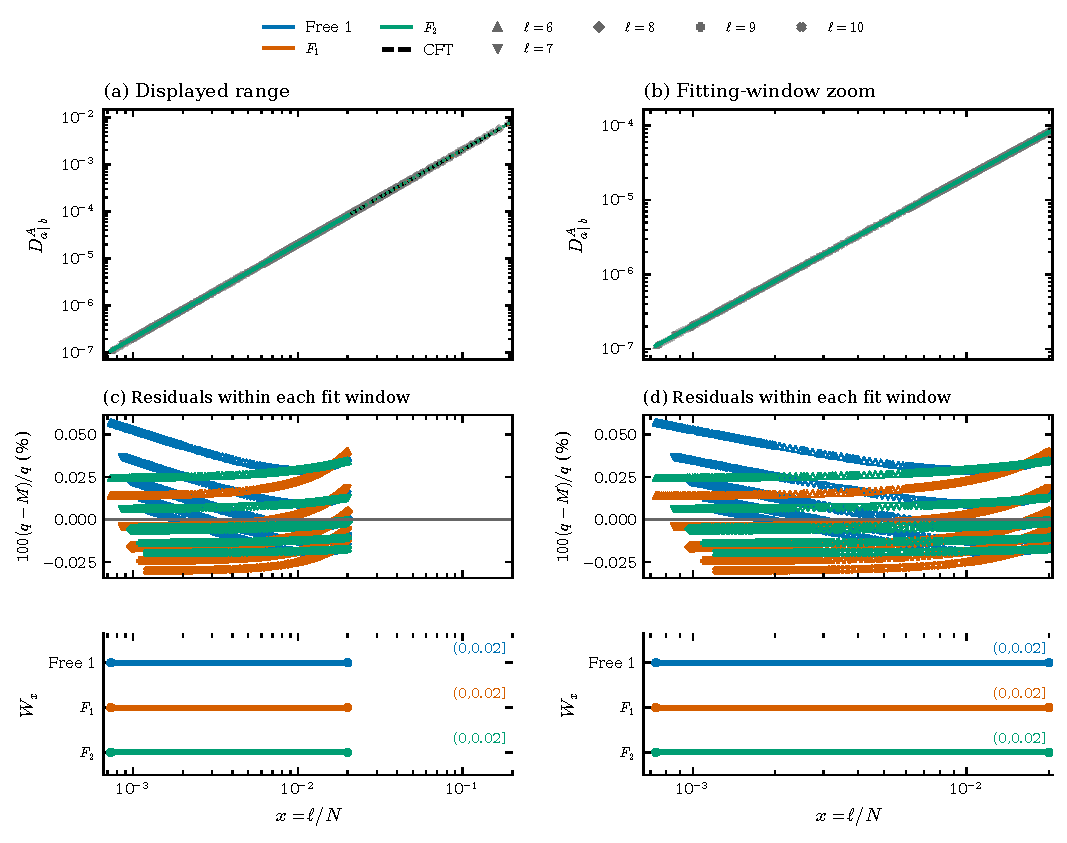
\includegraphics[width=.94\linewidth]{../figs/pair_small_ising_I_sigma.pdf}\par\smallskip
\begingroup\scriptsize\setlength{\tabcolsep}{4pt}
\begin{tabular}{lllrrrrr}\toprule
Set & Model & $W_z$ & $m$ & $c_0$ & $r^{(0)}$ & $c_1$ & $r^{(1)}$\\\midrule
Both & Free 1 & $(0,0.02]$ & 1255 & 0.20585 & 2.0001419 & --- & ---\\
Both & $F_1$ & $(0,0.02]$ & 1255 & 0.20573 & 2 & --- & ---\\
Both & $F_2$ & $(0,0.02]$ & 1255 & 0.20571 & 2 & 0.083833 & 4\\
\midrule
Both & CFT & --- & --- & 0.20562 & 2 & --- & ---\\
\bottomrule\end{tabular}
\endgroup
\caption{Ising, small intervals, $I\mid \sigma$, at $p=1/2$, $\ell=6,\ldots,10$, and the complete size grid in Eq.~\eqref{eq:extended-grid}. Here $z=x$ and $q=D^A$. Left: all computed data through $z=0.20$; right: a zoom into the common fitting window. Both columns show the same Free 1, $F_1$, and $F_2$ fits. All six directions of this CFT and interval type use the same window. Gray markers denote the data. Colored solid segments lie inside each model\textquotesingle s fitting interval; dotted segments are extrapolations. Black dashed is the supplied CFT series. The observable axes are logarithmic and span the measured data; nonpositive predictions cannot appear there and out-of-range extrapolations leave the panel. Residual ordinates are linear and show $100(q-M)/q$ only on each model\textquotesingle s fitted observations. Bars give the exact fitting intervals. The parameter block follows Eq.~\eqref{eq:fit}, with $c_0,c_1$ multiplying $z^{r^{(0)}},z^{r^{(1)}}$; all coefficients include powers of $\pi$. A dash means an absent fitted term, or no fitting window for CFT. Values shown are rounded; curves use full precision.}
\label{fig:pair-small_ising-I-sigma}
\end{figure}
\begin{figure}[!htbp]\centering
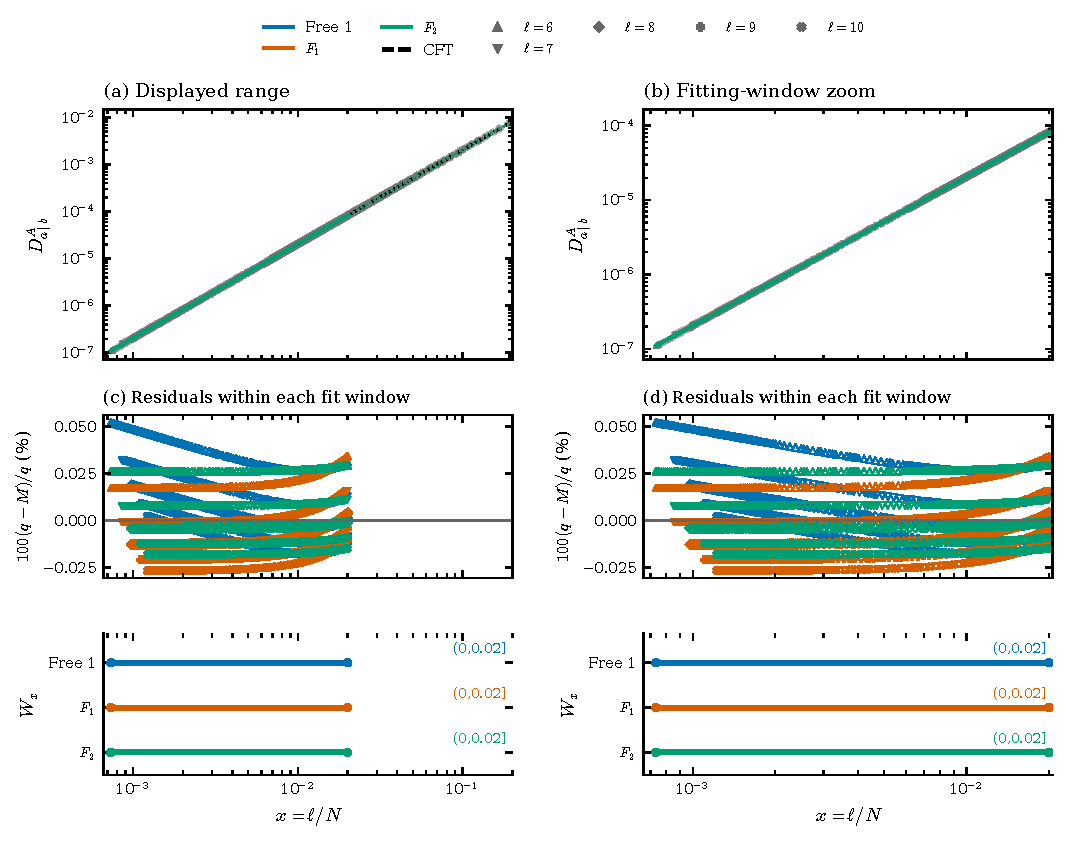
\includegraphics[width=.94\linewidth]{../figs/pair_small_ising_sigma_I.pdf}\par\smallskip
\begingroup\scriptsize\setlength{\tabcolsep}{4pt}
\begin{tabular}{lllrrrrr}\toprule
Set & Model & $W_z$ & $m$ & $c_0$ & $r^{(0)}$ & $c_1$ & $r^{(1)}$\\\midrule
Both & Free 1 & $(0,0.02]$ & 1255 & 0.20582 & 2.0001141 & --- & ---\\
Both & $F_1$ & $(0,0.02]$ & 1255 & 0.20572 & 2 & --- & ---\\
Both & $F_2$ & $(0,0.02]$ & 1255 & 0.2057 & 2 & 0.069099 & 4\\
\midrule
Both & CFT & --- & --- & 0.20562 & 2 & --- & ---\\
\bottomrule\end{tabular}
\endgroup
\caption{Ising, small intervals, $\sigma\mid I$, at $p=1/2$, $\ell=6,\ldots,10$, and the complete size grid in Eq.~\eqref{eq:extended-grid}. Here $z=x$ and $q=D^A$. Left: all computed data through $z=0.20$; right: a zoom into the common fitting window. Both columns show the same Free 1, $F_1$, and $F_2$ fits. All six directions of this CFT and interval type use the same window. Gray markers denote the data. Colored solid segments lie inside each model\textquotesingle s fitting interval; dotted segments are extrapolations. Black dashed is the supplied CFT series. The observable axes are logarithmic and span the measured data; nonpositive predictions cannot appear there and out-of-range extrapolations leave the panel. Residual ordinates are linear and show $100(q-M)/q$ only on each model\textquotesingle s fitted observations. Bars give the exact fitting intervals. The parameter block follows Eq.~\eqref{eq:fit}, with $c_0,c_1$ multiplying $z^{r^{(0)}},z^{r^{(1)}}$; all coefficients include powers of $\pi$. A dash means an absent fitted term, or no fitting window for CFT. Values shown are rounded; curves use full precision.}
\label{fig:pair-small_ising-sigma-I}
\end{figure}
\begin{figure}[!htbp]\centering
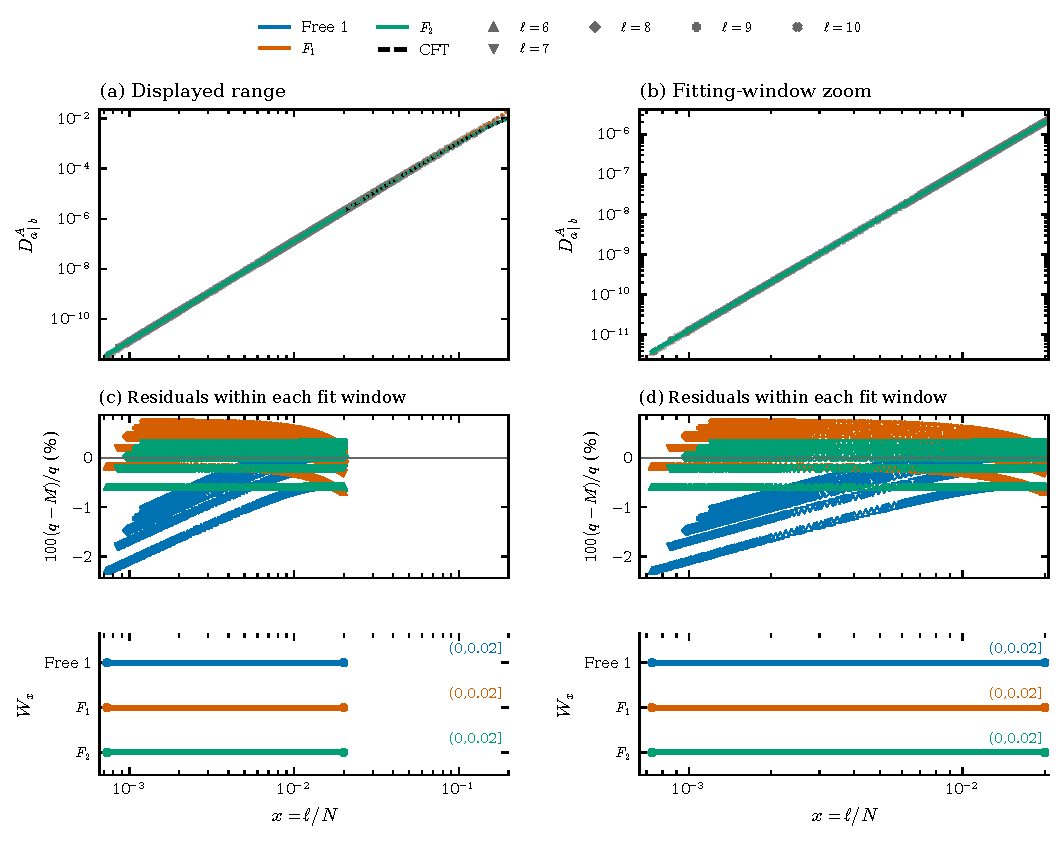
\includegraphics[width=.94\linewidth]{../figs/pair_small_ising_I_epsilon.pdf}\par\smallskip
\begingroup\scriptsize\setlength{\tabcolsep}{4pt}
\begin{tabular}{lllrrrrr}\toprule
Set & Model & $W_z$ & $m$ & $c_0$ & $r^{(0)}$ & $c_1$ & $r^{(1)}$\\\midrule
Both & Free 1 & $(0,0.02]$ & 1255 & 12.491 & 3.9933972 & --- & ---\\
Both & $F_1$ & $(0,0.02]$ & 1255 & 12.83 & 4 & --- & ---\\
Both & $F_2$ & $(0,0.02]$ & 1255 & 12.883 & 4 & -170.71 & 6\\
\midrule
Both & CFT & --- & --- & 12.988 & 4 & -170.91 & 6\\
\bottomrule\end{tabular}
\endgroup
\caption{Ising, small intervals, $I\mid \varepsilon$, at $p=1/2$, $\ell=6,\ldots,10$, and the complete size grid in Eq.~\eqref{eq:extended-grid}. Here $z=x$ and $q=D^A$. Left: all computed data through $z=0.20$; right: a zoom into the common fitting window. Both columns show the same Free 1, $F_1$, and $F_2$ fits. All six directions of this CFT and interval type use the same window. Gray markers denote the data. Colored solid segments lie inside each model\textquotesingle s fitting interval; dotted segments are extrapolations. Black dashed is the supplied CFT series. The observable axes are logarithmic and span the measured data; nonpositive predictions cannot appear there and out-of-range extrapolations leave the panel. Residual ordinates are linear and show $100(q-M)/q$ only on each model\textquotesingle s fitted observations. Bars give the exact fitting intervals. The parameter block follows Eq.~\eqref{eq:fit}, with $c_0,c_1$ multiplying $z^{r^{(0)}},z^{r^{(1)}}$; all coefficients include powers of $\pi$. A dash means an absent fitted term, or no fitting window for CFT. Values shown are rounded; curves use full precision.}
\label{fig:pair-small_ising-I-epsilon}
\end{figure}
\begin{figure}[!htbp]\centering
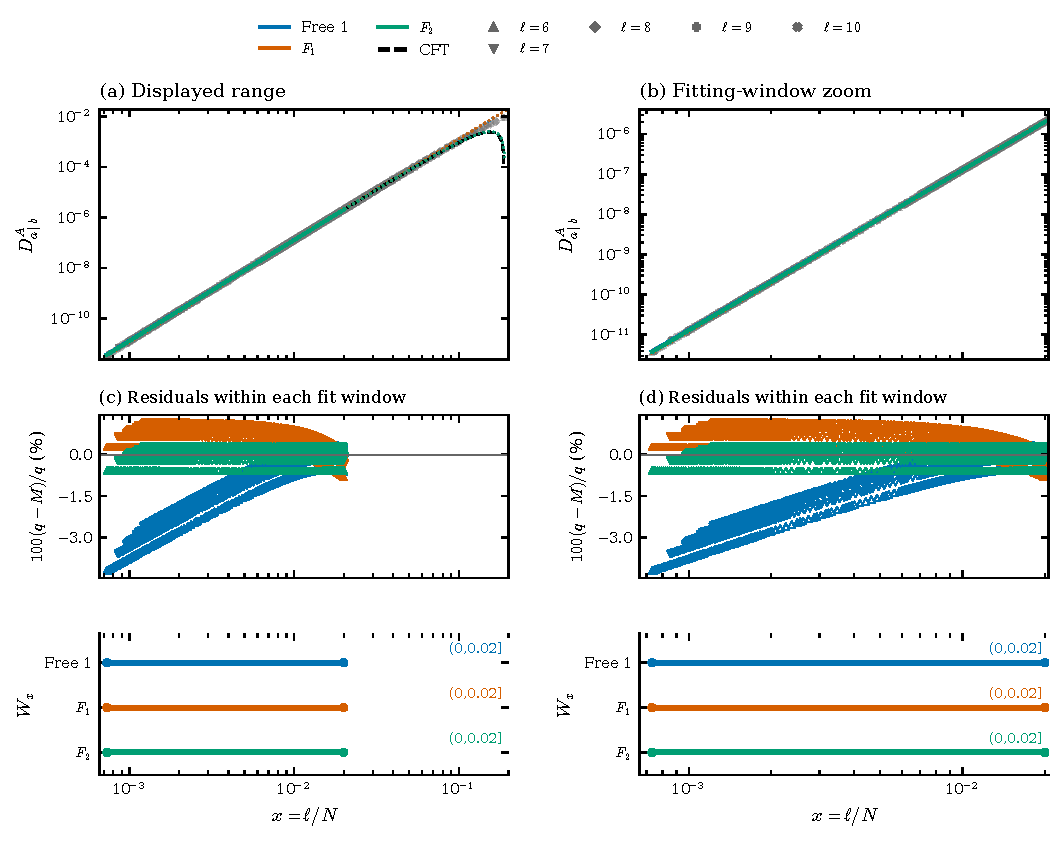
\includegraphics[width=.94\linewidth]{../figs/pair_small_ising_epsilon_I.pdf}\par\smallskip
\begingroup\scriptsize\setlength{\tabcolsep}{4pt}
\begin{tabular}{lllrrrrr}\toprule
Set & Model & $W_z$ & $m$ & $c_0$ & $r^{(0)}$ & $c_1$ & $r^{(1)}$\\\midrule
Both & Free 1 & $(0,0.02]$ & 1255 & 12.07 & 3.9860672 & --- & ---\\
Both & $F_1$ & $(0,0.02]$ & 1255 & 12.77 & 4 & --- & ---\\
Both & $F_2$ & $(0,0.02]$ & 1255 & 12.882 & 4 & -355.38 & 6\\
\midrule
Both & CFT & --- & --- & 12.988 & 4 & -366.24 & 6\\
\bottomrule\end{tabular}
\endgroup
\caption{Ising, small intervals, $\varepsilon\mid I$, at $p=1/2$, $\ell=6,\ldots,10$, and the complete size grid in Eq.~\eqref{eq:extended-grid}. Here $z=x$ and $q=D^A$. Left: all computed data through $z=0.20$; right: a zoom into the common fitting window. Both columns show the same Free 1, $F_1$, and $F_2$ fits. All six directions of this CFT and interval type use the same window. Gray markers denote the data. Colored solid segments lie inside each model\textquotesingle s fitting interval; dotted segments are extrapolations. Black dashed is the supplied CFT series. The observable axes are logarithmic and span the measured data; nonpositive predictions cannot appear there and out-of-range extrapolations leave the panel. Residual ordinates are linear and show $100(q-M)/q$ only on each model\textquotesingle s fitted observations. Bars give the exact fitting intervals. The parameter block follows Eq.~\eqref{eq:fit}, with $c_0,c_1$ multiplying $z^{r^{(0)}},z^{r^{(1)}}$; all coefficients include powers of $\pi$. A dash means an absent fitted term, or no fitting window for CFT. Values shown are rounded; curves use full precision.}
\label{fig:pair-small_ising-epsilon-I}
\end{figure}
\begin{figure}[!htbp]\centering
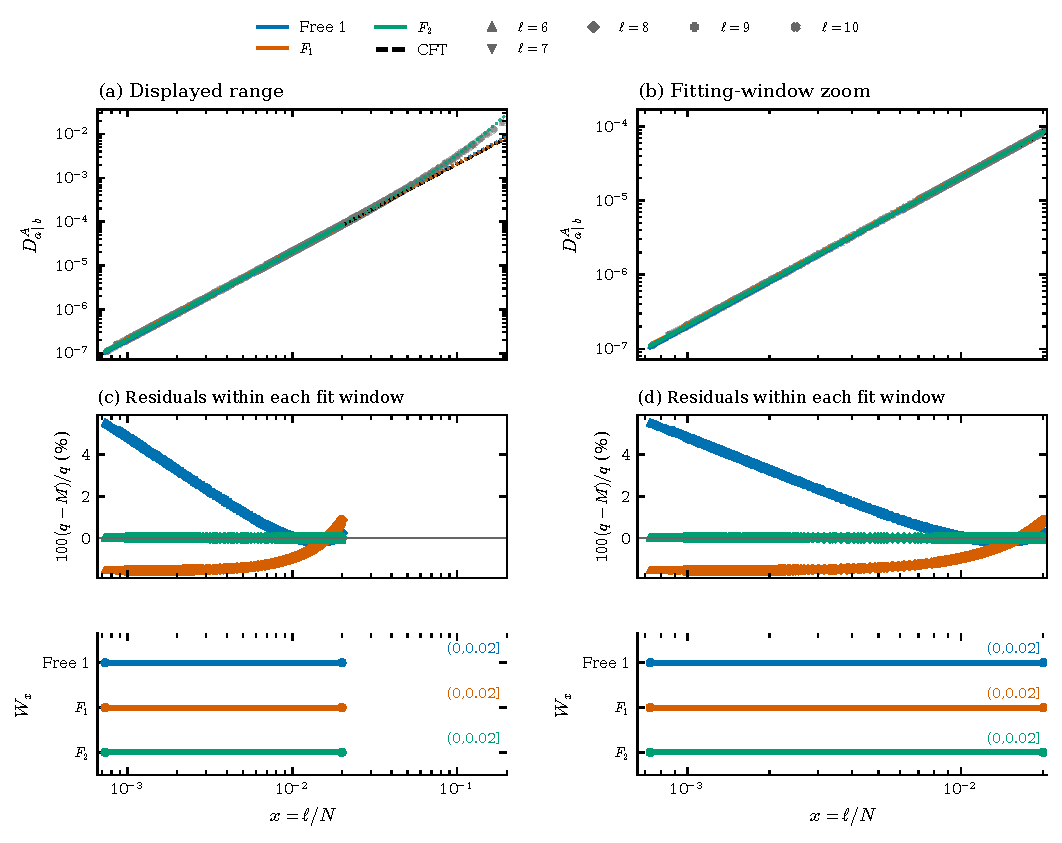
\includegraphics[width=.94\linewidth]{../figs/pair_small_ising_sigma_epsilon.pdf}\par\smallskip
\begingroup\scriptsize\setlength{\tabcolsep}{4pt}
\begin{tabular}{lllrrrrr}\toprule
Set & Model & $W_z$ & $m$ & $c_0$ & $r^{(0)}$ & $c_1$ & $r^{(1)}$\\\midrule
Both & Free 1 & $(0,0.02]$ & 1255 & 0.23069 & 2.0237554 & --- & ---\\
Both & $F_1$ & $(0,0.02]$ & 1255 & 0.2089 & 2 & --- & ---\\
Both & $F_2$ & $(0,0.02]$ & 1255 & 0.20565 & 2 & 12.604 & 4\\
\midrule
Both & CFT & --- & --- & 0.20562 & 2 & --- & ---\\
\bottomrule\end{tabular}
\endgroup
\caption{Ising, small intervals, $\sigma\mid \varepsilon$, at $p=1/2$, $\ell=6,\ldots,10$, and the complete size grid in Eq.~\eqref{eq:extended-grid}. Here $z=x$ and $q=D^A$. Left: all computed data through $z=0.20$; right: a zoom into the common fitting window. Both columns show the same Free 1, $F_1$, and $F_2$ fits. All six directions of this CFT and interval type use the same window. Gray markers denote the data. Colored solid segments lie inside each model\textquotesingle s fitting interval; dotted segments are extrapolations. Black dashed is the supplied CFT series. The observable axes are logarithmic and span the measured data; nonpositive predictions cannot appear there and out-of-range extrapolations leave the panel. Residual ordinates are linear and show $100(q-M)/q$ only on each model\textquotesingle s fitted observations. Bars give the exact fitting intervals. The parameter block follows Eq.~\eqref{eq:fit}, with $c_0,c_1$ multiplying $z^{r^{(0)}},z^{r^{(1)}}$; all coefficients include powers of $\pi$. A dash means an absent fitted term, or no fitting window for CFT. Values shown are rounded; curves use full precision.}
\label{fig:pair-small_ising-sigma-epsilon}
\end{figure}
\begin{figure}[!htbp]\centering
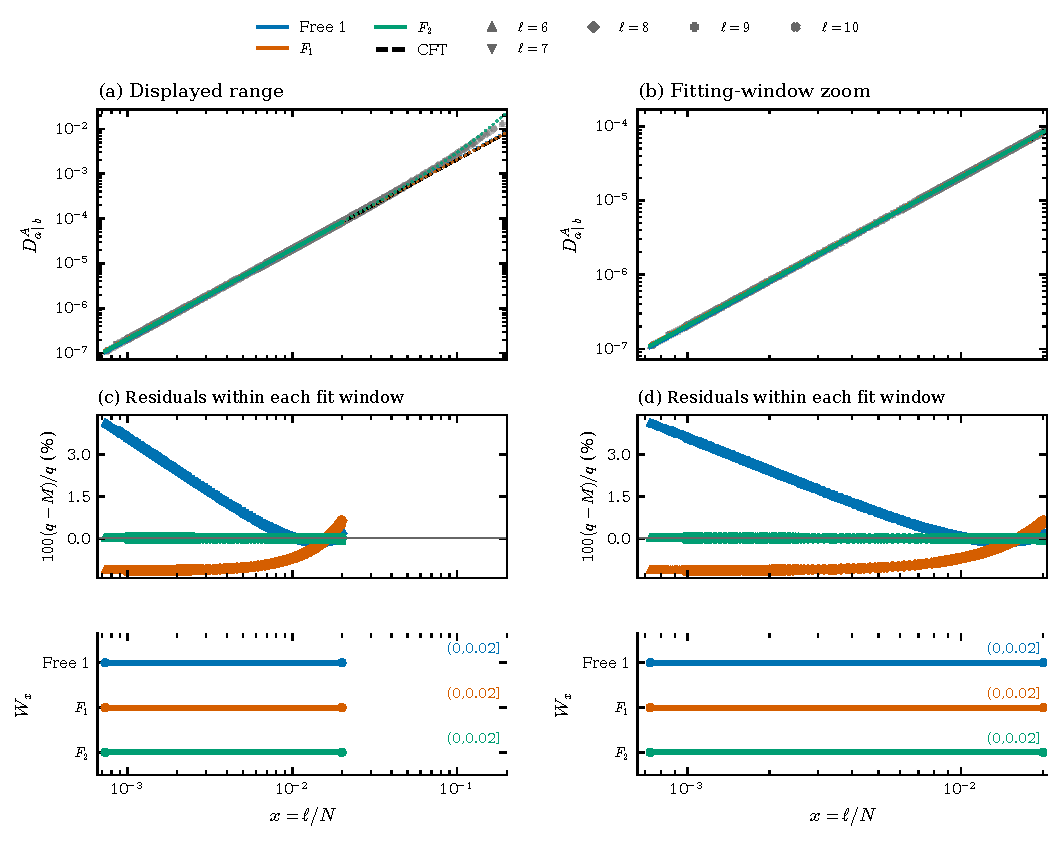
\includegraphics[width=.94\linewidth]{../figs/pair_small_ising_epsilon_sigma.pdf}\par\smallskip
\begingroup\scriptsize\setlength{\tabcolsep}{4pt}
\begin{tabular}{lllrrrrr}\toprule
Set & Model & $W_z$ & $m$ & $c_0$ & $r^{(0)}$ & $c_1$ & $r^{(1)}$\\\midrule
Both & Free 1 & $(0,0.02]$ & 1255 & 0.22393 & 2.0176011 & --- & ---\\
Both & $F_1$ & $(0,0.02]$ & 1255 & 0.20806 & 2 & --- & ---\\
Both & $F_2$ & $(0,0.02]$ & 1255 & 0.20566 & 2 & 9.3133 & 4\\
\midrule
Both & CFT & --- & --- & 0.20562 & 2 & --- & ---\\
\bottomrule\end{tabular}
\endgroup
\caption{Ising, small intervals, $\varepsilon\mid \sigma$, at $p=1/2$, $\ell=6,\ldots,10$, and the complete size grid in Eq.~\eqref{eq:extended-grid}. Here $z=x$ and $q=D^A$. Left: all computed data through $z=0.20$; right: a zoom into the common fitting window. Both columns show the same Free 1, $F_1$, and $F_2$ fits. All six directions of this CFT and interval type use the same window. Gray markers denote the data. Colored solid segments lie inside each model\textquotesingle s fitting interval; dotted segments are extrapolations. Black dashed is the supplied CFT series. The observable axes are logarithmic and span the measured data; nonpositive predictions cannot appear there and out-of-range extrapolations leave the panel. Residual ordinates are linear and show $100(q-M)/q$ only on each model\textquotesingle s fitted observations. Bars give the exact fitting intervals. The parameter block follows Eq.~\eqref{eq:fit}, with $c_0,c_1$ multiplying $z^{r^{(0)}},z^{r^{(1)}}$; all coefficients include powers of $\pi$. A dash means an absent fitted term, or no fitting window for CFT. Values shown are rounded; curves use full precision.}
\label{fig:pair-small_ising-epsilon-sigma}
\end{figure}

\clearpage
\subsection{Compact boson, small intervals}
\label{sec:pair-small_boson}
\begin{figure}[!htbp]\centering
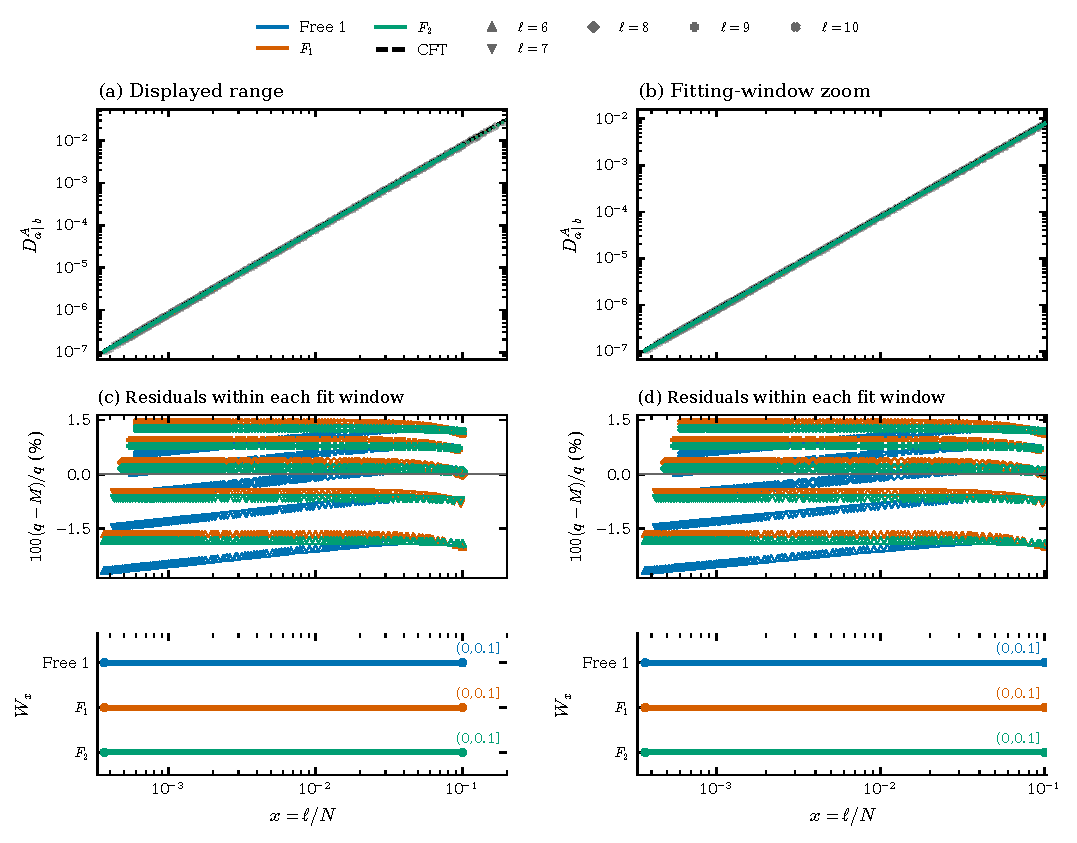
\includegraphics[width=.94\linewidth]{../figs/pair_small_boson_00_ss.pdf}\par\smallskip
\begingroup\scriptsize\setlength{\tabcolsep}{4pt}
\begin{tabular}{lllrrrrr}\toprule
Set & Model & $W_z$ & $m$ & $c_0$ & $r^{(0)}$ & $c_1$ & $r^{(1)}$\\\midrule
Both & Free 1 & $(0,0.1]$ & 598 & 0.77501 & 1.998159 & --- & ---\\
Both & $F_1$ & $(0,0.1]$ & 598 & 0.77866 & 2 & --- & ---\\
Both & $F_2$ & $(0,0.1]$ & 598 & 0.77996 & 2 & -0.1917 & 4\\
\midrule
Both & CFT & --- & --- & 0.82247 & 2 & --- & ---\\
\bottomrule\end{tabular}
\endgroup
\caption{Compact boson, small intervals, $00\mid ss$, at $p=1/2$, $\ell=6,\ldots,10$, and the complete size grid in Eq.~\eqref{eq:extended-grid}. Here $z=x$ and $q=D^A$. Left: all computed data through $z=0.20$; right: a zoom into the common fitting window. Both columns show the same Free 1, $F_1$, and $F_2$ fits. All six directions of this CFT and interval type use the same window. Gray markers denote the data. Colored solid segments lie inside each model\textquotesingle s fitting interval; dotted segments are extrapolations. Black dashed is the supplied CFT series. The observable axes are logarithmic and span the measured data; nonpositive predictions cannot appear there and out-of-range extrapolations leave the panel. Residual ordinates are linear and show $100(q-M)/q$ only on each model\textquotesingle s fitted observations. Bars give the exact fitting intervals. The parameter block follows Eq.~\eqref{eq:fit}, with $c_0,c_1$ multiplying $z^{r^{(0)}},z^{r^{(1)}}$; all coefficients include powers of $\pi$. A dash means an absent fitted term, or no fitting window for CFT. Values shown are rounded; curves use full precision.}
\label{fig:pair-small_boson-00-ss}
\end{figure}
\begin{figure}[!htbp]\centering
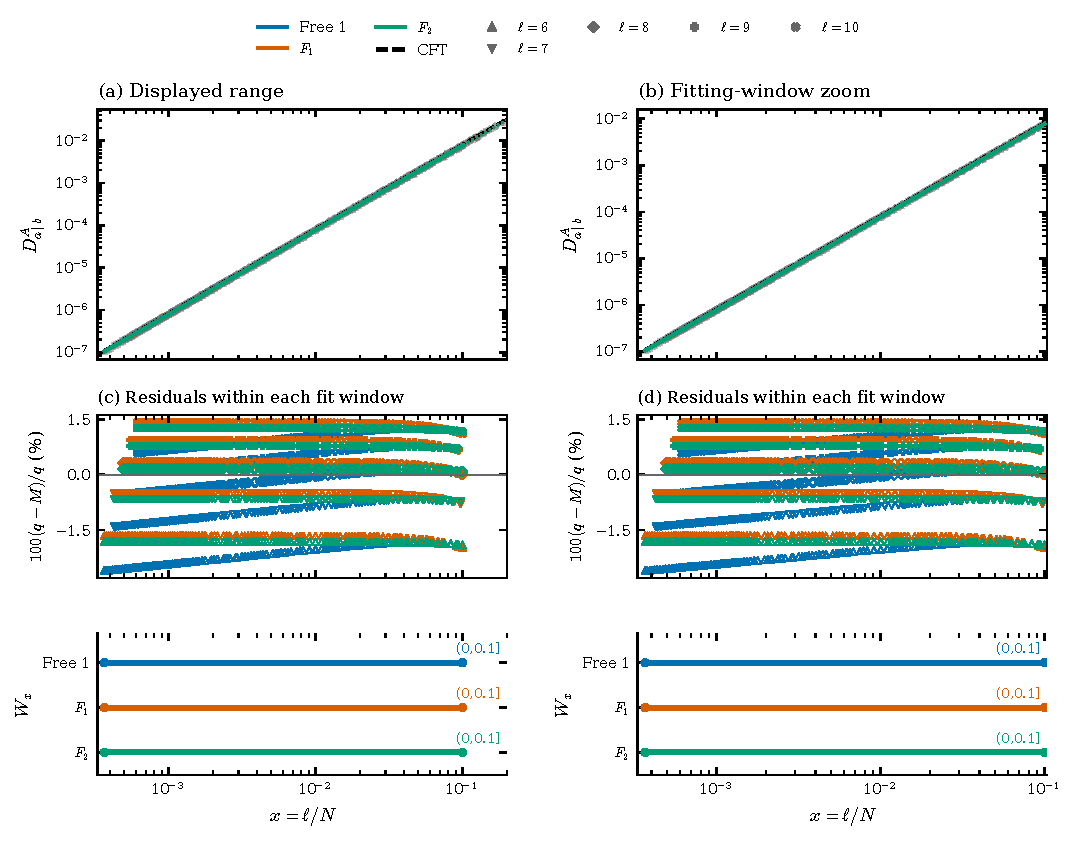
\includegraphics[width=.94\linewidth]{../figs/pair_small_boson_ss_00.pdf}\par\smallskip
\begingroup\scriptsize\setlength{\tabcolsep}{4pt}
\begin{tabular}{lllrrrrr}\toprule
Set & Model & $W_z$ & $m$ & $c_0$ & $r^{(0)}$ & $c_1$ & $r^{(1)}$\\\midrule
Both & Free 1 & $(0,0.1]$ & 598 & 0.77529 & 1.9982698 & --- & ---\\
Both & $F_1$ & $(0,0.1]$ & 598 & 0.77871 & 2 & --- & ---\\
Both & $F_2$ & $(0,0.1]$ & 598 & 0.77995 & 2 & -0.18219 & 4\\
\midrule
Both & CFT & --- & --- & 0.82247 & 2 & --- & ---\\
\bottomrule\end{tabular}
\endgroup
\caption{Compact boson, small intervals, $ss\mid 00$, at $p=1/2$, $\ell=6,\ldots,10$, and the complete size grid in Eq.~\eqref{eq:extended-grid}. Here $z=x$ and $q=D^A$. Left: all computed data through $z=0.20$; right: a zoom into the common fitting window. Both columns show the same Free 1, $F_1$, and $F_2$ fits. All six directions of this CFT and interval type use the same window. Gray markers denote the data. Colored solid segments lie inside each model\textquotesingle s fitting interval; dotted segments are extrapolations. Black dashed is the supplied CFT series. The observable axes are logarithmic and span the measured data; nonpositive predictions cannot appear there and out-of-range extrapolations leave the panel. Residual ordinates are linear and show $100(q-M)/q$ only on each model\textquotesingle s fitted observations. Bars give the exact fitting intervals. The parameter block follows Eq.~\eqref{eq:fit}, with $c_0,c_1$ multiplying $z^{r^{(0)}},z^{r^{(1)}}$; all coefficients include powers of $\pi$. A dash means an absent fitted term, or no fitting window for CFT. Values shown are rounded; curves use full precision.}
\label{fig:pair-small_boson-ss-00}
\end{figure}
\begin{figure}[!htbp]\centering
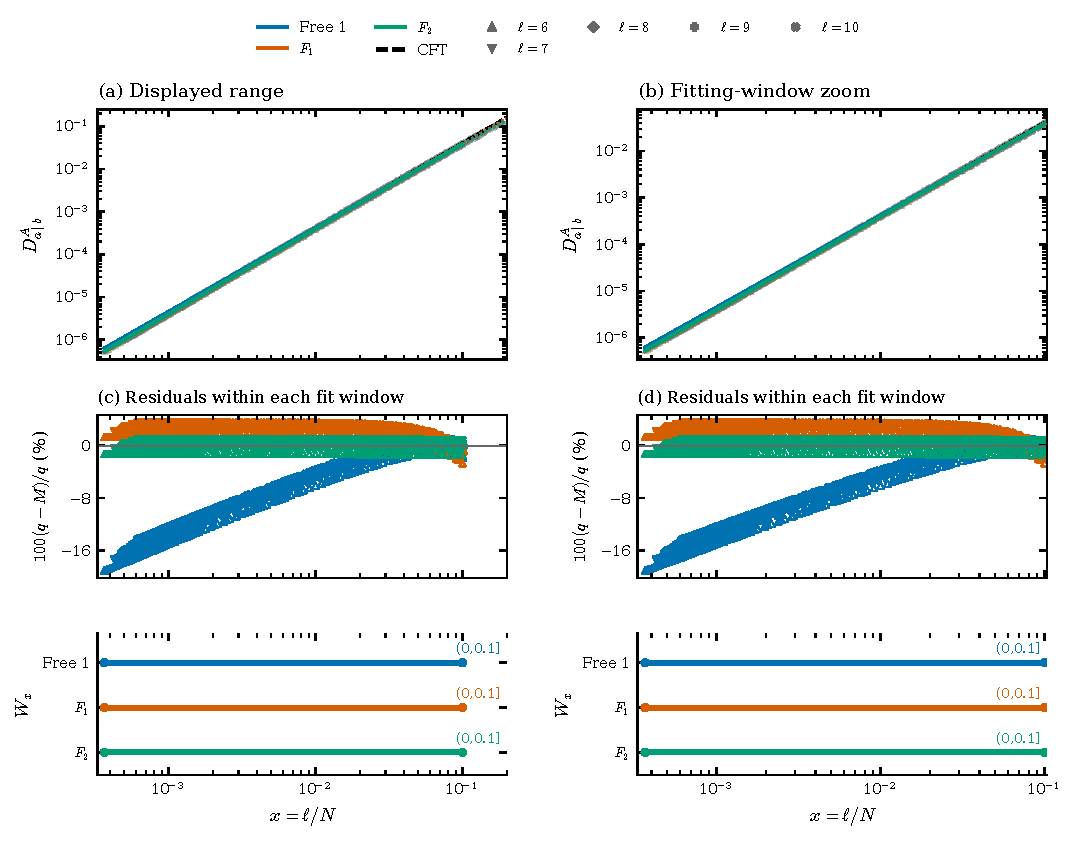
\includegraphics[width=.94\linewidth]{../figs/pair_small_boson_00_3s_s.pdf}\par\smallskip
\begingroup\scriptsize\setlength{\tabcolsep}{4pt}
\begin{tabular}{lllrrrrr}\toprule
Set & Model & $W_z$ & $m$ & $c_0$ & $r^{(0)}$ & $c_1$ & $r^{(1)}$\\\midrule
Both & Free 1 & $(0,0.1]$ & 598 & 3.5315 & 1.9648776 & --- & ---\\
Both & $F_1$ & $(0,0.1]$ & 598 & 3.8623 & 2 & --- & ---\\
Both & $F_2$ & $(0,0.1]$ & 598 & 3.964 & 2 & -15.02 & 4\\
\midrule
Both & CFT & --- & --- & 4.1123 & 2 & --- & ---\\
\bottomrule\end{tabular}
\endgroup
\caption{Compact boson, small intervals, $00\mid 3s,s$, at $p=1/2$, $\ell=6,\ldots,10$, and the complete size grid in Eq.~\eqref{eq:extended-grid}. Here $z=x$ and $q=D^A$. Left: all computed data through $z=0.20$; right: a zoom into the common fitting window. Both columns show the same Free 1, $F_1$, and $F_2$ fits. All six directions of this CFT and interval type use the same window. Gray markers denote the data. Colored solid segments lie inside each model\textquotesingle s fitting interval; dotted segments are extrapolations. Black dashed is the supplied CFT series. The observable axes are logarithmic and span the measured data; nonpositive predictions cannot appear there and out-of-range extrapolations leave the panel. Residual ordinates are linear and show $100(q-M)/q$ only on each model\textquotesingle s fitted observations. Bars give the exact fitting intervals. The parameter block follows Eq.~\eqref{eq:fit}, with $c_0,c_1$ multiplying $z^{r^{(0)}},z^{r^{(1)}}$; all coefficients include powers of $\pi$. A dash means an absent fitted term, or no fitting window for CFT. Values shown are rounded; curves use full precision.}
\label{fig:pair-small_boson-00-3s_s}
\end{figure}
\begin{figure}[!htbp]\centering
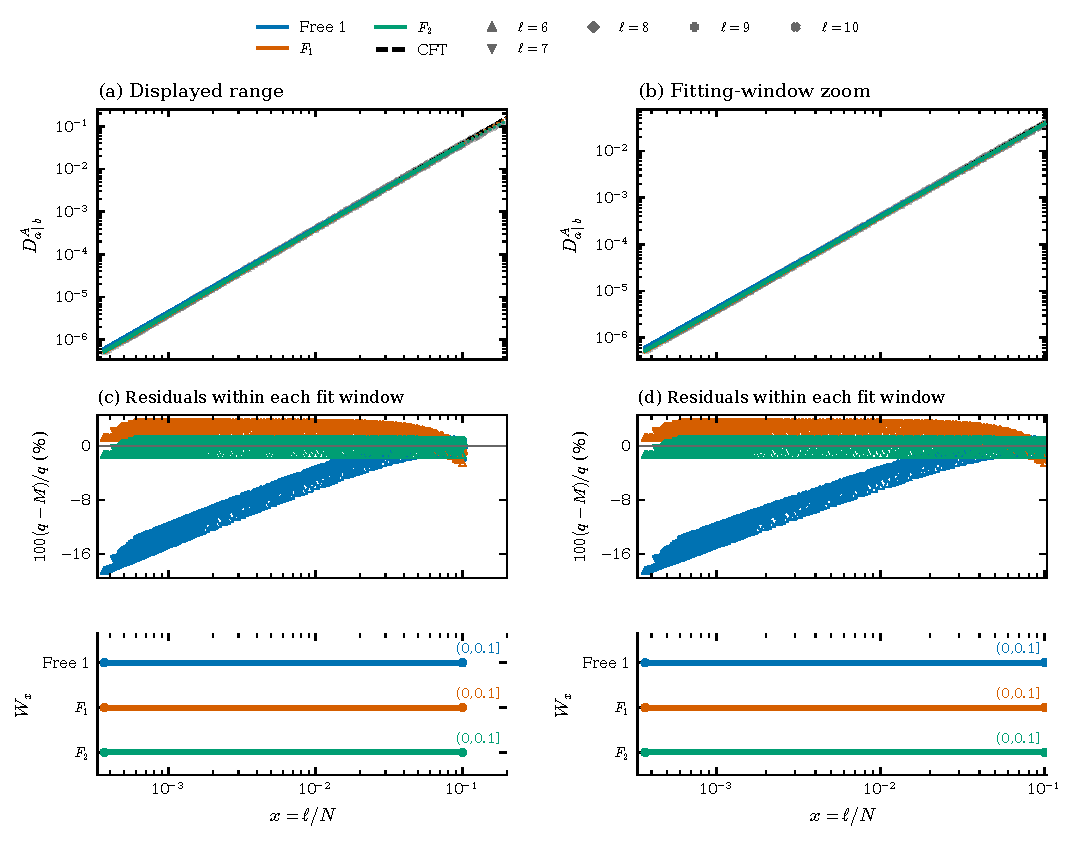
\includegraphics[width=.94\linewidth]{../figs/pair_small_boson_3s_s_00.pdf}\par\smallskip
\begingroup\scriptsize\setlength{\tabcolsep}{4pt}
\begin{tabular}{lllrrrrr}\toprule
Set & Model & $W_z$ & $m$ & $c_0$ & $r^{(0)}$ & $c_1$ & $r^{(1)}$\\\midrule
Both & Free 1 & $(0,0.1]$ & 598 & 3.545 & 1.9660249 & --- & ---\\
Both & $F_1$ & $(0,0.1]$ & 598 & 3.8657 & 2 & --- & ---\\
Both & $F_2$ & $(0,0.1]$ & 598 & 3.9643 & 2 & -14.541 & 4\\
\midrule
Both & CFT & --- & --- & 4.1123 & 2 & --- & ---\\
\bottomrule\end{tabular}
\endgroup
\caption{Compact boson, small intervals, $3s,s\mid 00$, at $p=1/2$, $\ell=6,\ldots,10$, and the complete size grid in Eq.~\eqref{eq:extended-grid}. Here $z=x$ and $q=D^A$. Left: all computed data through $z=0.20$; right: a zoom into the common fitting window. Both columns show the same Free 1, $F_1$, and $F_2$ fits. All six directions of this CFT and interval type use the same window. Gray markers denote the data. Colored solid segments lie inside each model\textquotesingle s fitting interval; dotted segments are extrapolations. Black dashed is the supplied CFT series. The observable axes are logarithmic and span the measured data; nonpositive predictions cannot appear there and out-of-range extrapolations leave the panel. Residual ordinates are linear and show $100(q-M)/q$ only on each model\textquotesingle s fitted observations. Bars give the exact fitting intervals. The parameter block follows Eq.~\eqref{eq:fit}, with $c_0,c_1$ multiplying $z^{r^{(0)}},z^{r^{(1)}}$; all coefficients include powers of $\pi$. A dash means an absent fitted term, or no fitting window for CFT. Values shown are rounded; curves use full precision.}
\label{fig:pair-small_boson-3s_s-00}
\end{figure}
\begin{figure}[!htbp]\centering
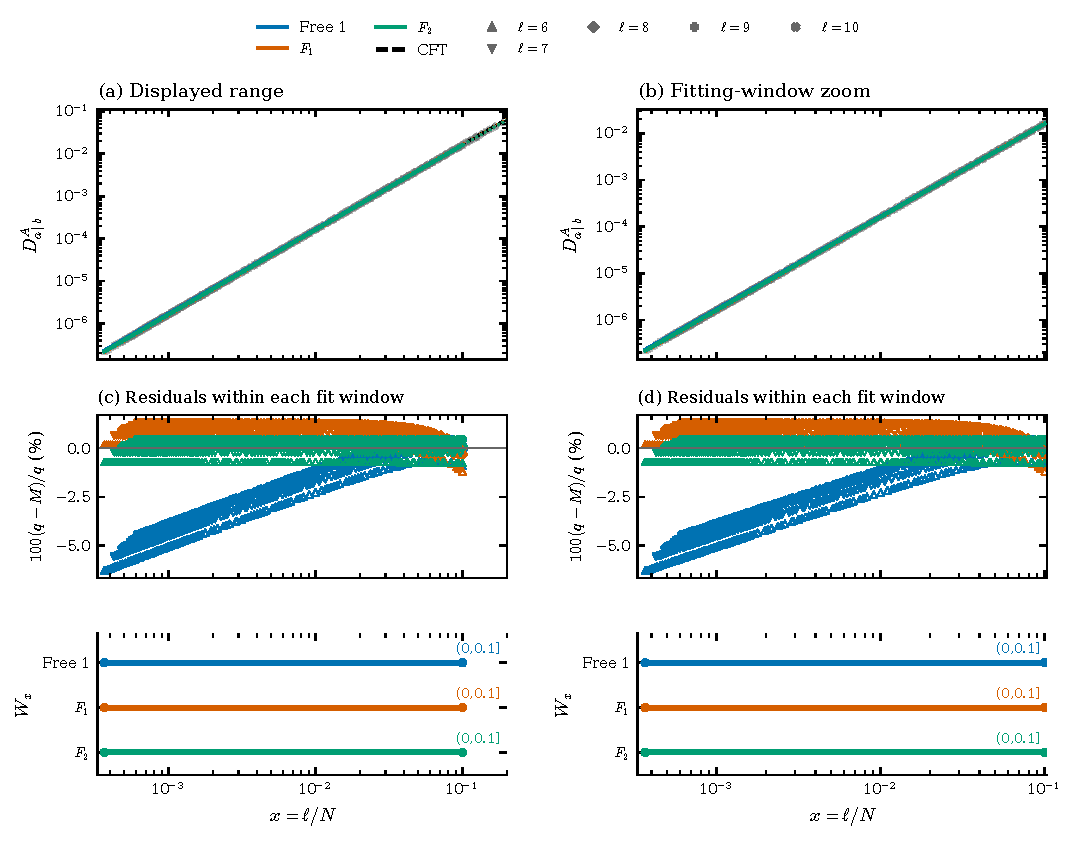
\includegraphics[width=.94\linewidth]{../figs/pair_small_boson_ss_3s_s.pdf}\par\smallskip
\begingroup\scriptsize\setlength{\tabcolsep}{4pt}
\begin{tabular}{lllrrrrr}\toprule
Set & Model & $W_z$ & $m$ & $c_0$ & $r^{(0)}$ & $c_1$ & $r^{(1)}$\\\midrule
Both & Free 1 & $(0,0.1]$ & 598 & 1.5661 & 1.9883068 & --- & ---\\
Both & $F_1$ & $(0,0.1]$ & 598 & 1.6134 & 2 & --- & ---\\
Both & $F_2$ & $(0,0.1]$ & 598 & 1.6276 & 2 & -2.0896 & 4\\
\midrule
Both & CFT & --- & --- & 1.6449 & 2 & --- & ---\\
\bottomrule\end{tabular}
\endgroup
\caption{Compact boson, small intervals, $ss\mid 3s,s$, at $p=1/2$, $\ell=6,\ldots,10$, and the complete size grid in Eq.~\eqref{eq:extended-grid}. Here $z=x$ and $q=D^A$. Left: all computed data through $z=0.20$; right: a zoom into the common fitting window. Both columns show the same Free 1, $F_1$, and $F_2$ fits. All six directions of this CFT and interval type use the same window. Gray markers denote the data. Colored solid segments lie inside each model\textquotesingle s fitting interval; dotted segments are extrapolations. Black dashed is the supplied CFT series. The observable axes are logarithmic and span the measured data; nonpositive predictions cannot appear there and out-of-range extrapolations leave the panel. Residual ordinates are linear and show $100(q-M)/q$ only on each model\textquotesingle s fitted observations. Bars give the exact fitting intervals. The parameter block follows Eq.~\eqref{eq:fit}, with $c_0,c_1$ multiplying $z^{r^{(0)}},z^{r^{(1)}}$; all coefficients include powers of $\pi$. A dash means an absent fitted term, or no fitting window for CFT. Values shown are rounded; curves use full precision.}
\label{fig:pair-small_boson-ss-3s_s}
\end{figure}
\begin{figure}[!htbp]\centering
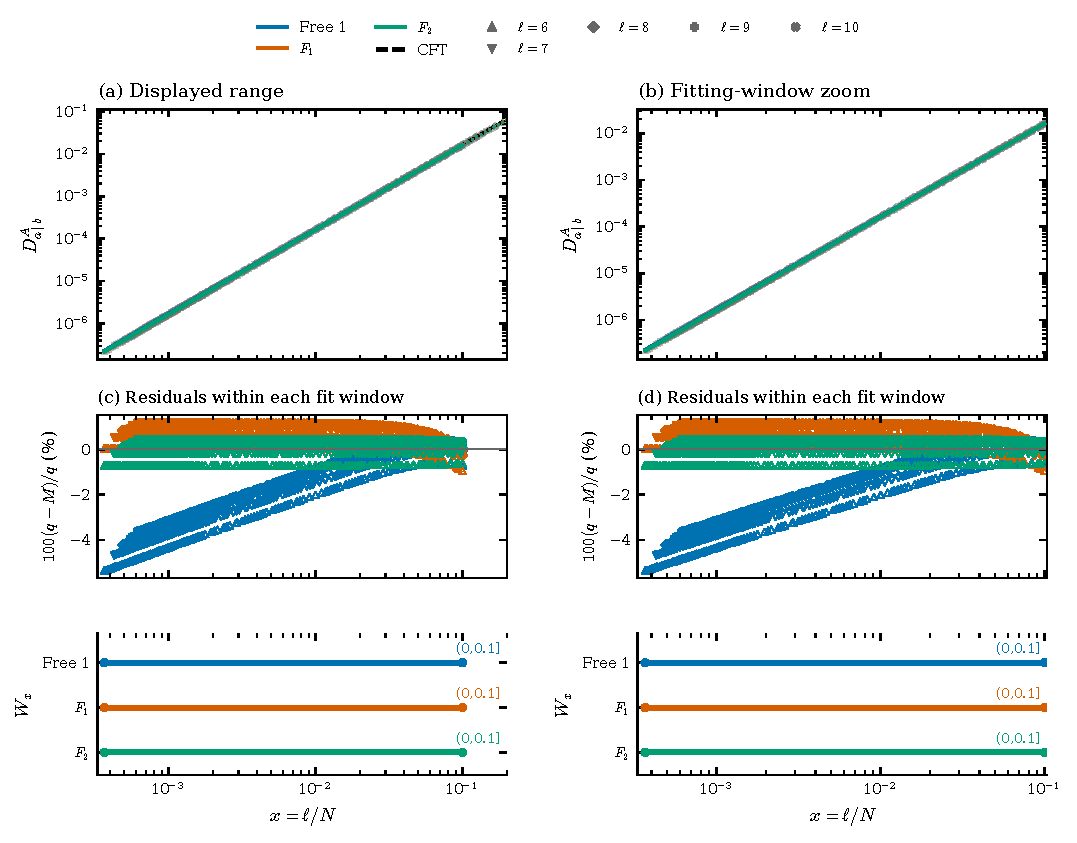
\includegraphics[width=.94\linewidth]{../figs/pair_small_boson_3s_s_ss.pdf}\par\smallskip
\begingroup\scriptsize\setlength{\tabcolsep}{4pt}
\begin{tabular}{lllrrrrr}\toprule
Set & Model & $W_z$ & $m$ & $c_0$ & $r^{(0)}$ & $c_1$ & $r^{(1)}$\\\midrule
Both & Free 1 & $(0,0.1]$ & 598 & 1.576 & 1.9902202 & --- & ---\\
Both & $F_1$ & $(0,0.1]$ & 598 & 1.6157 & 2 & --- & ---\\
Both & $F_2$ & $(0,0.1]$ & 598 & 1.6276 & 2 & -1.7507 & 4\\
\midrule
Both & CFT & --- & --- & 1.6449 & 2 & --- & ---\\
\bottomrule\end{tabular}
\endgroup
\caption{Compact boson, small intervals, $3s,s\mid ss$, at $p=1/2$, $\ell=6,\ldots,10$, and the complete size grid in Eq.~\eqref{eq:extended-grid}. Here $z=x$ and $q=D^A$. Left: all computed data through $z=0.20$; right: a zoom into the common fitting window. Both columns show the same Free 1, $F_1$, and $F_2$ fits. All six directions of this CFT and interval type use the same window. Gray markers denote the data. Colored solid segments lie inside each model\textquotesingle s fitting interval; dotted segments are extrapolations. Black dashed is the supplied CFT series. The observable axes are logarithmic and span the measured data; nonpositive predictions cannot appear there and out-of-range extrapolations leave the panel. Residual ordinates are linear and show $100(q-M)/q$ only on each model\textquotesingle s fitted observations. Bars give the exact fitting intervals. The parameter block follows Eq.~\eqref{eq:fit}, with $c_0,c_1$ multiplying $z^{r^{(0)}},z^{r^{(1)}}$; all coefficients include powers of $\pi$. A dash means an absent fitted term, or no fitting window for CFT. Values shown are rounded; curves use full precision.}
\label{fig:pair-small_boson-3s_s-ss}
\end{figure}

\clearpage
\subsection{Ising, large intervals}
\label{sec:pair-large_ising}
\begin{figure}[!htbp]\centering
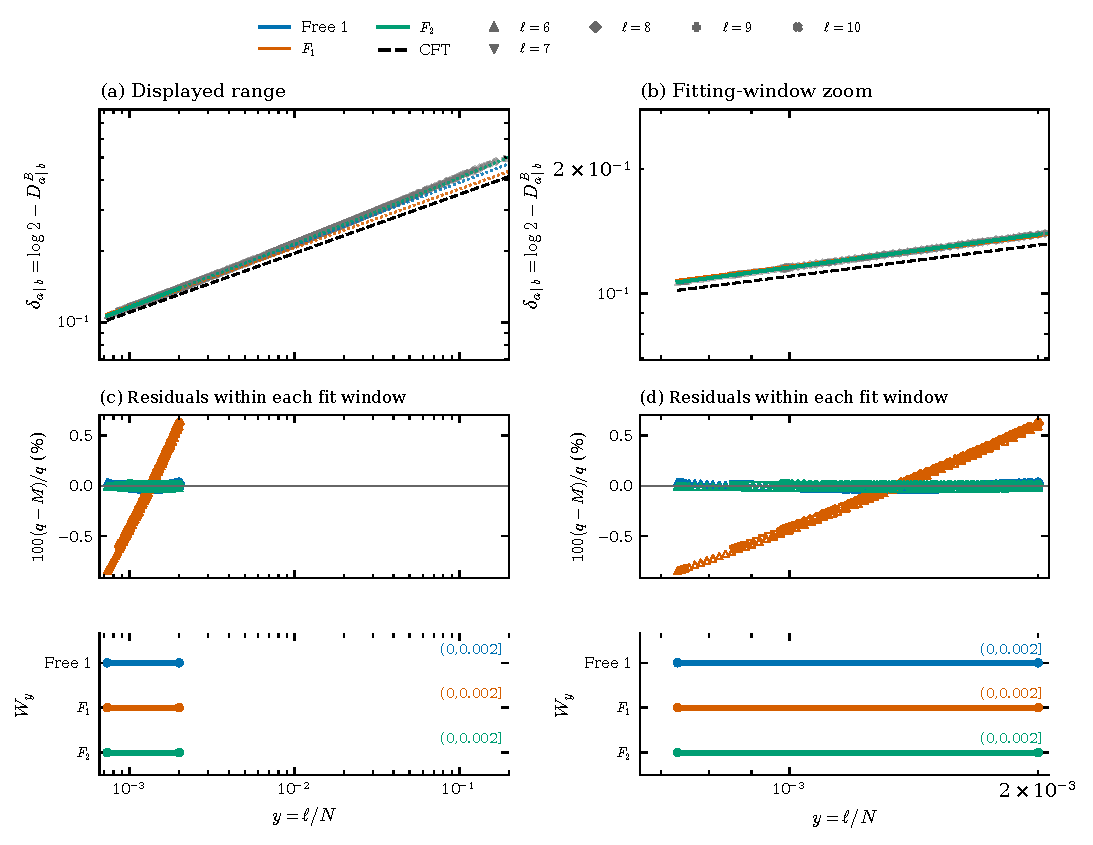
\includegraphics[width=.94\linewidth]{../figs/pair_large_ising_I_sigma.pdf}\par\smallskip
\begingroup\scriptsize\setlength{\tabcolsep}{4pt}
\begin{tabular}{lllrrrrr}\toprule
Set & Model & $W_z$ & $m$ & $c_0$ & $r^{(0)}$ & $c_1$ & $r^{(1)}$\\\midrule
Both & Free 1 & $(0,0.002]$ & 260 & 0.71994 & 0.2646516 & --- & ---\\
Both & $F_1$ & $(0,0.002]$ & 260 & 0.65339 & 0.25 & --- & ---\\
Both & $F_2$ & $(0,0.002]$ & 260 & 0.61463 & 0.25 & 0.20243 & 0.5\\
\midrule
Both & CFT & --- & --- & 0.61965 & 0.25 & --- & ---\\
\bottomrule\end{tabular}
\endgroup
\caption{Ising, large intervals, $I\mid \sigma$, at $p=1/2$, $\ell=6,\ldots,10$, and the complete size grid in Eq.~\eqref{eq:extended-grid}. Here $z=y$ and $q=\delta=\log2-D^B$. Left: all computed data through $z=0.20$; right: a zoom into the common fitting window. Both columns show the same Free 1, $F_1$, and $F_2$ fits. All six directions of this CFT and interval type use the same window. Gray markers denote the data. Colored solid segments lie inside each model\textquotesingle s fitting interval; dotted segments are extrapolations. Black dashed is the analytical CFT leading deficit. The observable axes are logarithmic and span the measured data; nonpositive predictions cannot appear there and out-of-range extrapolations leave the panel. Residual ordinates are linear and show $100(q-M)/q$ only on each model\textquotesingle s fitted observations. Bars give the exact fitting intervals. The parameter block follows Eq.~\eqref{eq:fit}, with $c_0,c_1$ multiplying $z^{r^{(0)}},z^{r^{(1)}}$; all coefficients include powers of $\pi$. A dash means an absent fitted term, or no fitting window for CFT. Values shown are rounded; curves use full precision.}
\label{fig:pair-large_ising-I-sigma}
\end{figure}
\begin{figure}[!htbp]\centering
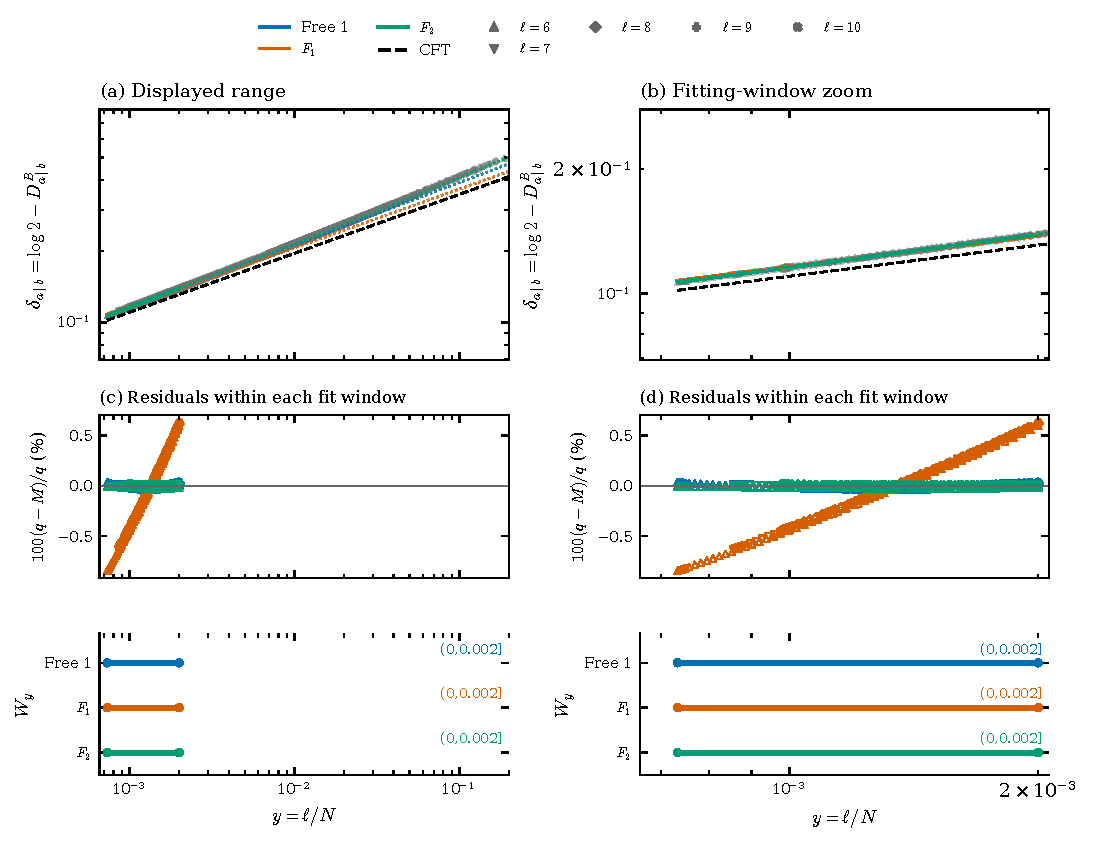
\includegraphics[width=.94\linewidth]{../figs/pair_large_ising_sigma_I.pdf}\par\smallskip
\begingroup\scriptsize\setlength{\tabcolsep}{4pt}
\begin{tabular}{lllrrrrr}\toprule
Set & Model & $W_z$ & $m$ & $c_0$ & $r^{(0)}$ & $c_1$ & $r^{(1)}$\\\midrule
Both & Free 1 & $(0,0.002]$ & 260 & 0.71995 & 0.2646531 & --- & ---\\
Both & $F_1$ & $(0,0.002]$ & 260 & 0.65339 & 0.25 & --- & ---\\
Both & $F_2$ & $(0,0.002]$ & 260 & 0.61462 & 0.25 & 0.20245 & 0.5\\
\midrule
Both & CFT & --- & --- & 0.61965 & 0.25 & --- & ---\\
\bottomrule\end{tabular}
\endgroup
\caption{Ising, large intervals, $\sigma\mid I$, at $p=1/2$, $\ell=6,\ldots,10$, and the complete size grid in Eq.~\eqref{eq:extended-grid}. Here $z=y$ and $q=\delta=\log2-D^B$. Left: all computed data through $z=0.20$; right: a zoom into the common fitting window. Both columns show the same Free 1, $F_1$, and $F_2$ fits. All six directions of this CFT and interval type use the same window. Gray markers denote the data. Colored solid segments lie inside each model\textquotesingle s fitting interval; dotted segments are extrapolations. Black dashed is the analytical CFT leading deficit. The observable axes are logarithmic and span the measured data; nonpositive predictions cannot appear there and out-of-range extrapolations leave the panel. Residual ordinates are linear and show $100(q-M)/q$ only on each model\textquotesingle s fitted observations. Bars give the exact fitting intervals. The parameter block follows Eq.~\eqref{eq:fit}, with $c_0,c_1$ multiplying $z^{r^{(0)}},z^{r^{(1)}}$; all coefficients include powers of $\pi$. A dash means an absent fitted term, or no fitting window for CFT. Values shown are rounded; curves use full precision.}
\label{fig:pair-large_ising-sigma-I}
\end{figure}
\begin{figure}[!htbp]\centering
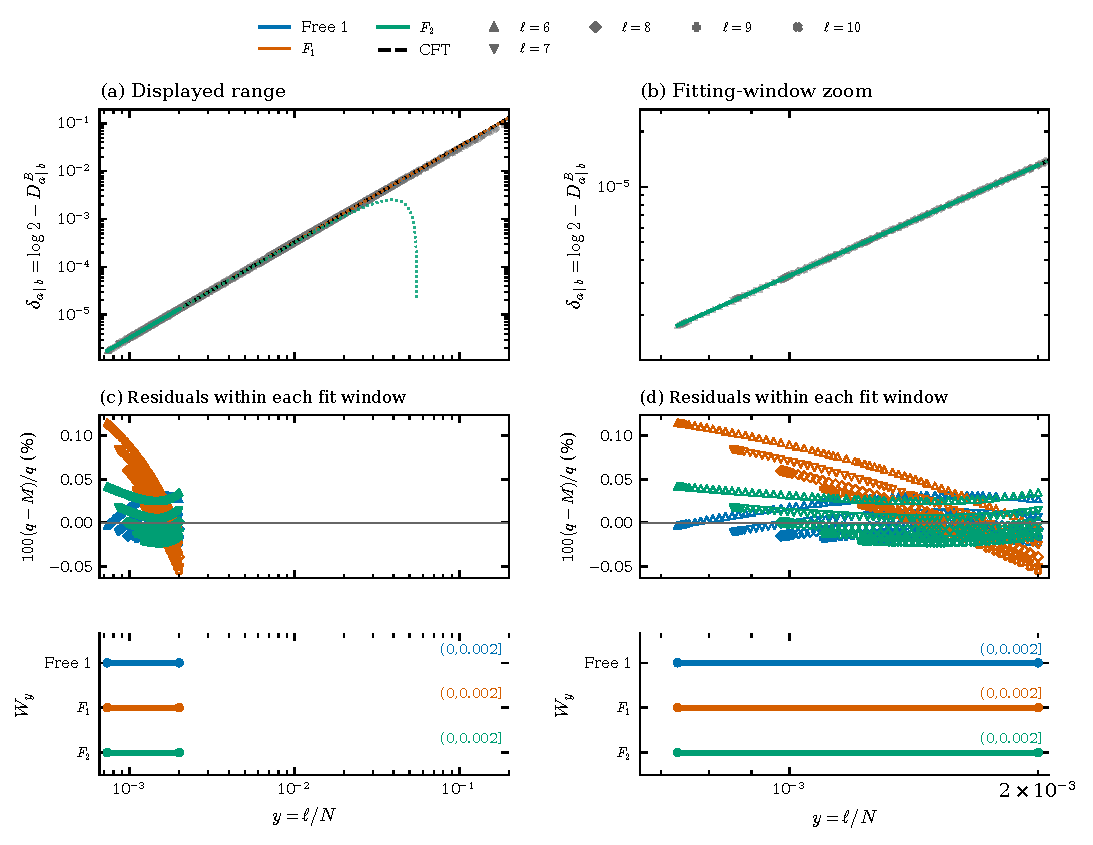
\includegraphics[width=.94\linewidth]{../figs/pair_large_ising_I_epsilon.pdf}\par\smallskip
\begingroup\scriptsize\setlength{\tabcolsep}{4pt}
\begin{tabular}{lllrrrrr}\toprule
Set & Model & $W_z$ & $m$ & $c_0$ & $r^{(0)}$ & $c_1$ & $r^{(1)}$\\\midrule
Both & Free 1 & $(0,0.002]$ & 260 & 3.2548 & 1.9985103 & --- & ---\\
Both & $F_1$ & $(0,0.002]$ & 260 & 3.2861 & 2 & --- & ---\\
Both & $F_2$ & $(0,0.002]$ & 260 & 3.289 & 2 & -1070.2 & 4\\
\midrule
Both & CFT & --- & --- & 3.2899 & 2 & --- & ---\\
\bottomrule\end{tabular}
\endgroup
\caption{Ising, large intervals, $I\mid \varepsilon$, at $p=1/2$, $\ell=6,\ldots,10$, and the complete size grid in Eq.~\eqref{eq:extended-grid}. Here $z=y$ and $q=\delta=\log2-D^B$. Left: all computed data through $z=0.20$; right: a zoom into the common fitting window. Both columns show the same Free 1, $F_1$, and $F_2$ fits. All six directions of this CFT and interval type use the same window. Gray markers denote the data. Colored solid segments lie inside each model\textquotesingle s fitting interval; dotted segments are extrapolations. Black dashed is the analytical CFT leading deficit. The observable axes are logarithmic and span the measured data; nonpositive predictions cannot appear there and out-of-range extrapolations leave the panel. Residual ordinates are linear and show $100(q-M)/q$ only on each model\textquotesingle s fitted observations. Bars give the exact fitting intervals. The parameter block follows Eq.~\eqref{eq:fit}, with $c_0,c_1$ multiplying $z^{r^{(0)}},z^{r^{(1)}}$; all coefficients include powers of $\pi$. A dash means an absent fitted term, or no fitting window for CFT. Values shown are rounded; curves use full precision.}
\label{fig:pair-large_ising-I-epsilon}
\end{figure}
\begin{figure}[!htbp]\centering
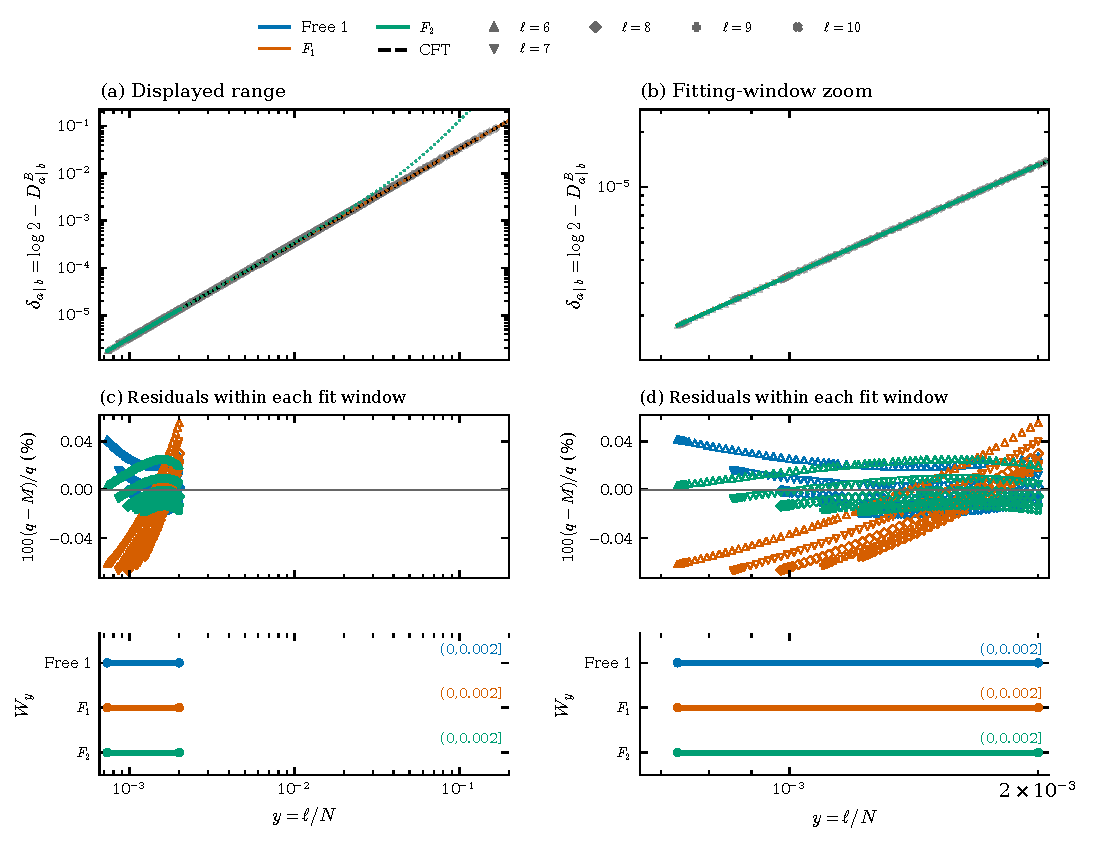
\includegraphics[width=.94\linewidth]{../figs/pair_large_ising_epsilon_I.pdf}\par\smallskip
\begingroup\scriptsize\setlength{\tabcolsep}{4pt}
\begin{tabular}{lllrrrrr}\toprule
Set & Model & $W_z$ & $m$ & $c_0$ & $r^{(0)}$ & $c_1$ & $r^{(1)}$\\\midrule
Both & Free 1 & $(0,0.002]$ & 260 & 3.3242 & 2.0013063 & --- & ---\\
Both & $F_1$ & $(0,0.002]$ & 260 & 3.2964 & 2 & --- & ---\\
Both & $F_2$ & $(0,0.002]$ & 260 & 3.2938 & 2 & 959.21 & 4\\
\midrule
Both & CFT & --- & --- & 3.2899 & 2 & --- & ---\\
\bottomrule\end{tabular}
\endgroup
\caption{Ising, large intervals, $\varepsilon\mid I$, at $p=1/2$, $\ell=6,\ldots,10$, and the complete size grid in Eq.~\eqref{eq:extended-grid}. Here $z=y$ and $q=\delta=\log2-D^B$. Left: all computed data through $z=0.20$; right: a zoom into the common fitting window. Both columns show the same Free 1, $F_1$, and $F_2$ fits. All six directions of this CFT and interval type use the same window. Gray markers denote the data. Colored solid segments lie inside each model\textquotesingle s fitting interval; dotted segments are extrapolations. Black dashed is the analytical CFT leading deficit. The observable axes are logarithmic and span the measured data; nonpositive predictions cannot appear there and out-of-range extrapolations leave the panel. Residual ordinates are linear and show $100(q-M)/q$ only on each model\textquotesingle s fitted observations. Bars give the exact fitting intervals. The parameter block follows Eq.~\eqref{eq:fit}, with $c_0,c_1$ multiplying $z^{r^{(0)}},z^{r^{(1)}}$; all coefficients include powers of $\pi$. A dash means an absent fitted term, or no fitting window for CFT. Values shown are rounded; curves use full precision.}
\label{fig:pair-large_ising-epsilon-I}
\end{figure}
\begin{figure}[!htbp]\centering
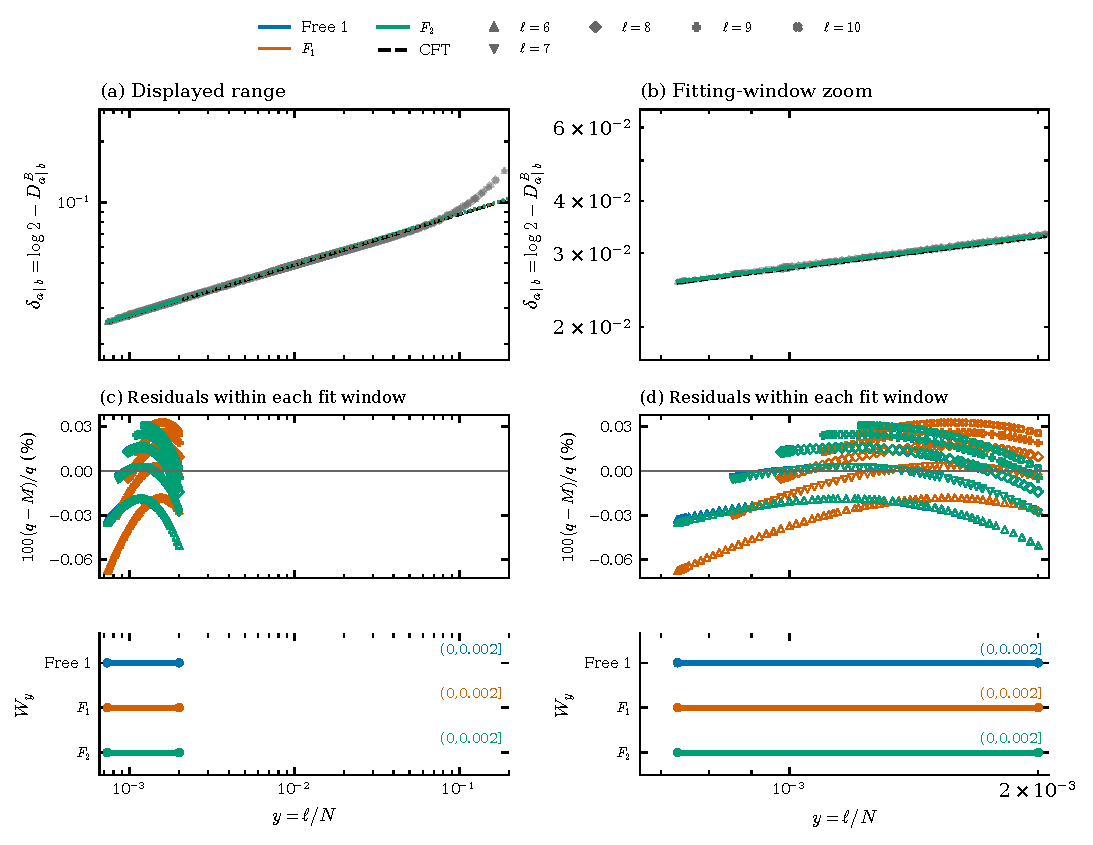
\includegraphics[width=.94\linewidth]{../figs/pair_large_ising_sigma_epsilon.pdf}\par\smallskip
\begingroup\scriptsize\setlength{\tabcolsep}{4pt}
\begin{tabular}{lllrrrrr}\toprule
Set & Model & $W_z$ & $m$ & $c_0$ & $r^{(0)}$ & $c_1$ & $r^{(1)}$\\\midrule
Both & Free 1 & $(0,0.002]$ & 260 & 0.15691 & 0.2505807 & --- & ---\\
Both & $F_1$ & $(0,0.002]$ & 260 & 0.15631 & 0.25 & --- & ---\\
Both & $F_2$ & $(0,0.002]$ & 260 & 0.15595 & 0.25 & 0.0018716 & 0.5\\
\midrule
Both & CFT & --- & --- & 0.15491 & 0.25 & --- & ---\\
\bottomrule\end{tabular}
\endgroup
\caption{Ising, large intervals, $\sigma\mid \varepsilon$, at $p=1/2$, $\ell=6,\ldots,10$, and the complete size grid in Eq.~\eqref{eq:extended-grid}. Here $z=y$ and $q=\delta=\log2-D^B$. Left: all computed data through $z=0.20$; right: a zoom into the common fitting window. Both columns show the same Free 1, $F_1$, and $F_2$ fits. All six directions of this CFT and interval type use the same window. Gray markers denote the data. Colored solid segments lie inside each model\textquotesingle s fitting interval; dotted segments are extrapolations. Black dashed is the analytical CFT leading deficit. The observable axes are logarithmic and span the measured data; nonpositive predictions cannot appear there and out-of-range extrapolations leave the panel. Residual ordinates are linear and show $100(q-M)/q$ only on each model\textquotesingle s fitted observations. Bars give the exact fitting intervals. The parameter block follows Eq.~\eqref{eq:fit}, with $c_0,c_1$ multiplying $z^{r^{(0)}},z^{r^{(1)}}$; all coefficients include powers of $\pi$. A dash means an absent fitted term, or no fitting window for CFT. Values shown are rounded; curves use full precision.}
\label{fig:pair-large_ising-sigma-epsilon}
\end{figure}
\begin{figure}[!htbp]\centering
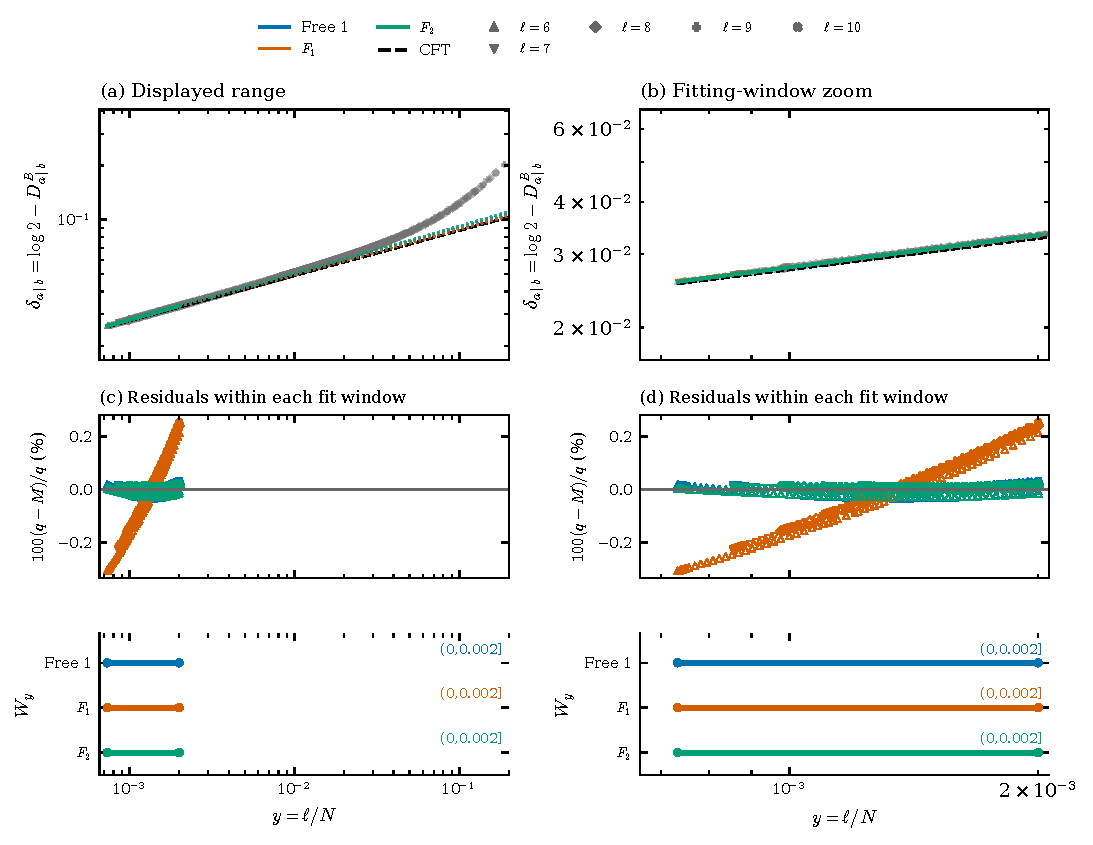
\includegraphics[width=.94\linewidth]{../figs/pair_large_ising_epsilon_sigma.pdf}\par\smallskip
\begingroup\scriptsize\setlength{\tabcolsep}{4pt}
\begin{tabular}{lllrrrrr}\toprule
Set & Model & $W_z$ & $m$ & $c_0$ & $r^{(0)}$ & $c_1$ & $r^{(1)}$\\\midrule
Both & Free 1 & $(0,0.002]$ & 260 & 0.16288 & 0.2554384 & --- & ---\\
Both & $F_1$ & $(0,0.002]$ & 260 & 0.15712 & 0.25 & --- & ---\\
Both & $F_2$ & $(0,0.002]$ & 260 & 0.15365 & 0.25 & 0.018087 & 0.5\\
\midrule
Both & CFT & --- & --- & 0.15491 & 0.25 & --- & ---\\
\bottomrule\end{tabular}
\endgroup
\caption{Ising, large intervals, $\varepsilon\mid \sigma$, at $p=1/2$, $\ell=6,\ldots,10$, and the complete size grid in Eq.~\eqref{eq:extended-grid}. Here $z=y$ and $q=\delta=\log2-D^B$. Left: all computed data through $z=0.20$; right: a zoom into the common fitting window. Both columns show the same Free 1, $F_1$, and $F_2$ fits. All six directions of this CFT and interval type use the same window. Gray markers denote the data. Colored solid segments lie inside each model\textquotesingle s fitting interval; dotted segments are extrapolations. Black dashed is the analytical CFT leading deficit. The observable axes are logarithmic and span the measured data; nonpositive predictions cannot appear there and out-of-range extrapolations leave the panel. Residual ordinates are linear and show $100(q-M)/q$ only on each model\textquotesingle s fitted observations. Bars give the exact fitting intervals. The parameter block follows Eq.~\eqref{eq:fit}, with $c_0,c_1$ multiplying $z^{r^{(0)}},z^{r^{(1)}}$; all coefficients include powers of $\pi$. A dash means an absent fitted term, or no fitting window for CFT. Values shown are rounded; curves use full precision.}
\label{fig:pair-large_ising-epsilon-sigma}
\end{figure}

\clearpage
\subsection{Compact boson, large intervals}
\label{sec:pair-large_boson}
\begin{figure}[!htbp]\centering
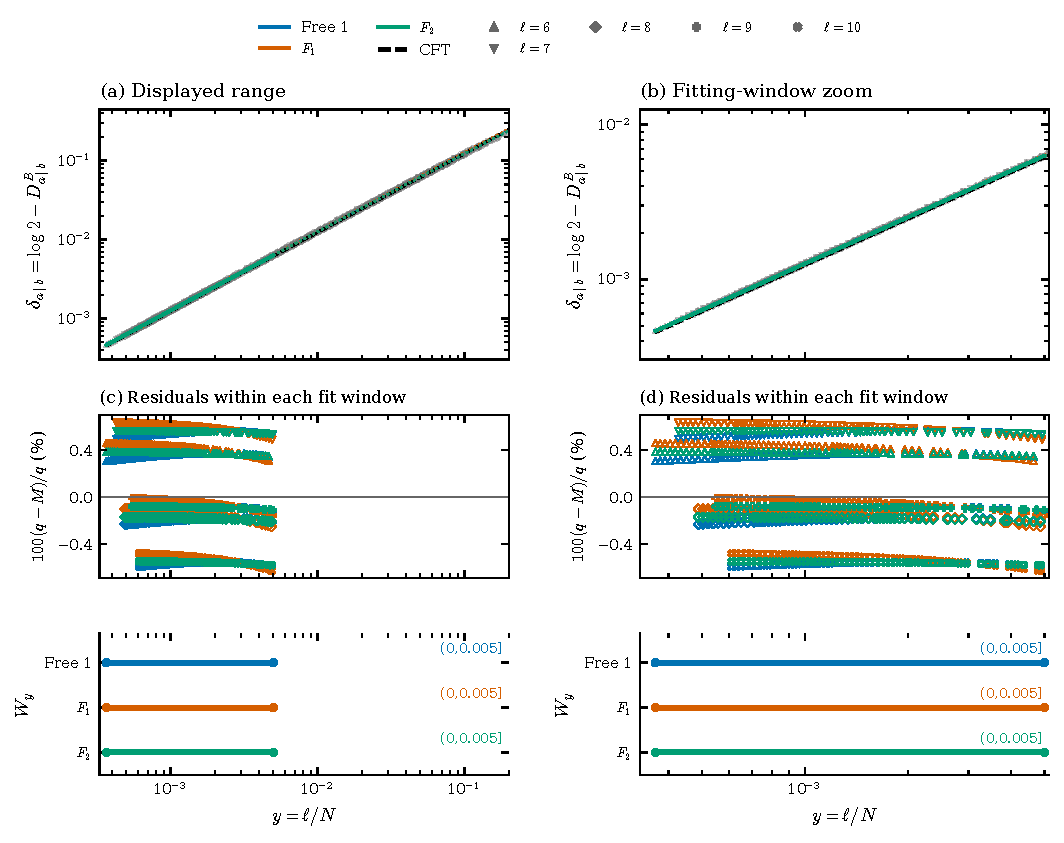
\includegraphics[width=.94\linewidth]{../figs/pair_large_boson_00_ss.pdf}\par\smallskip
\begingroup\scriptsize\setlength{\tabcolsep}{4pt}
\begin{tabular}{lllrrrrr}\toprule
Set & Model & $W_z$ & $m$ & $c_0$ & $r^{(0)}$ & $c_1$ & $r^{(1)}$\\\midrule
Both & Free 1 & $(0,0.005]$ & 317 & 1.2561 & 0.9992554 & --- & ---\\
Both & $F_1$ & $(0,0.005]$ & 317 & 1.2616 & 1 & --- & ---\\
Both & $F_2$ & $(0,0.005]$ & 317 & 1.2627 & 1 & -0.33376 & 2\\
\midrule
Both & CFT & --- & --- & 1.2337 & 1 & --- & ---\\
\bottomrule\end{tabular}
\endgroup
\caption{Compact boson, large intervals, $00\mid ss$, at $p=1/2$, $\ell=6,\ldots,10$, and the complete size grid in Eq.~\eqref{eq:extended-grid}. Here $z=y$ and $q=\delta=\log2-D^B$. Left: all computed data through $z=0.20$; right: a zoom into the common fitting window. Both columns show the same Free 1, $F_1$, and $F_2$ fits. All six directions of this CFT and interval type use the same window. Gray markers denote the data. Colored solid segments lie inside each model\textquotesingle s fitting interval; dotted segments are extrapolations. Black dashed is the analytical CFT leading deficit. The observable axes are logarithmic and span the measured data; nonpositive predictions cannot appear there and out-of-range extrapolations leave the panel. Residual ordinates are linear and show $100(q-M)/q$ only on each model\textquotesingle s fitted observations. Bars give the exact fitting intervals. The parameter block follows Eq.~\eqref{eq:fit}, with $c_0,c_1$ multiplying $z^{r^{(0)}},z^{r^{(1)}}$; all coefficients include powers of $\pi$. A dash means an absent fitted term, or no fitting window for CFT. Values shown are rounded; curves use full precision.}
\label{fig:pair-large_boson-00-ss}
\end{figure}
\begin{figure}[!htbp]\centering
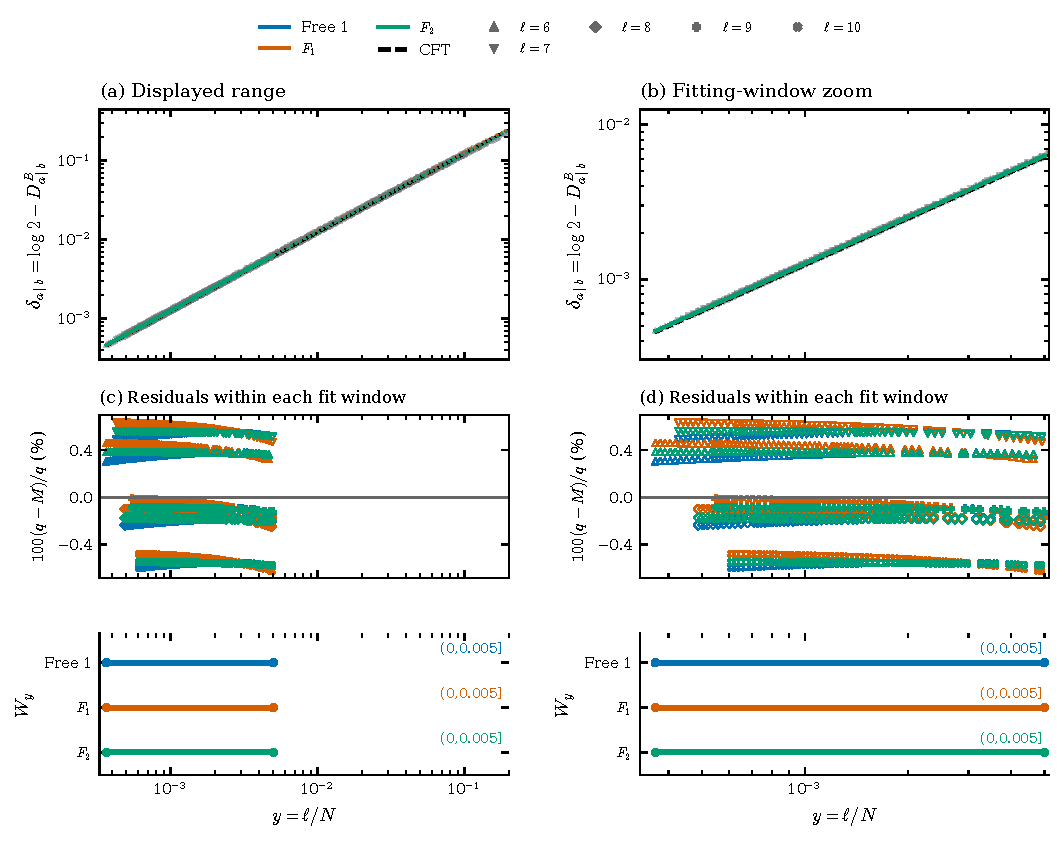
\includegraphics[width=.94\linewidth]{../figs/pair_large_boson_ss_00.pdf}\par\smallskip
\begingroup\scriptsize\setlength{\tabcolsep}{4pt}
\begin{tabular}{lllrrrrr}\toprule
Set & Model & $W_z$ & $m$ & $c_0$ & $r^{(0)}$ & $c_1$ & $r^{(1)}$\\\midrule
Both & Free 1 & $(0,0.005]$ & 317 & 1.256 & 0.9992434 & --- & ---\\
Both & $F_1$ & $(0,0.005]$ & 317 & 1.2616 & 1 & --- & ---\\
Both & $F_2$ & $(0,0.005]$ & 317 & 1.2627 & 1 & -0.34138 & 2\\
\midrule
Both & CFT & --- & --- & 1.2337 & 1 & --- & ---\\
\bottomrule\end{tabular}
\endgroup
\caption{Compact boson, large intervals, $ss\mid 00$, at $p=1/2$, $\ell=6,\ldots,10$, and the complete size grid in Eq.~\eqref{eq:extended-grid}. Here $z=y$ and $q=\delta=\log2-D^B$. Left: all computed data through $z=0.20$; right: a zoom into the common fitting window. Both columns show the same Free 1, $F_1$, and $F_2$ fits. All six directions of this CFT and interval type use the same window. Gray markers denote the data. Colored solid segments lie inside each model\textquotesingle s fitting interval; dotted segments are extrapolations. Black dashed is the analytical CFT leading deficit. The observable axes are logarithmic and span the measured data; nonpositive predictions cannot appear there and out-of-range extrapolations leave the panel. Residual ordinates are linear and show $100(q-M)/q$ only on each model\textquotesingle s fitted observations. Bars give the exact fitting intervals. The parameter block follows Eq.~\eqref{eq:fit}, with $c_0,c_1$ multiplying $z^{r^{(0)}},z^{r^{(1)}}$; all coefficients include powers of $\pi$. A dash means an absent fitted term, or no fitting window for CFT. Values shown are rounded; curves use full precision.}
\label{fig:pair-large_boson-ss-00}
\end{figure}
\begin{figure}[!htbp]\centering
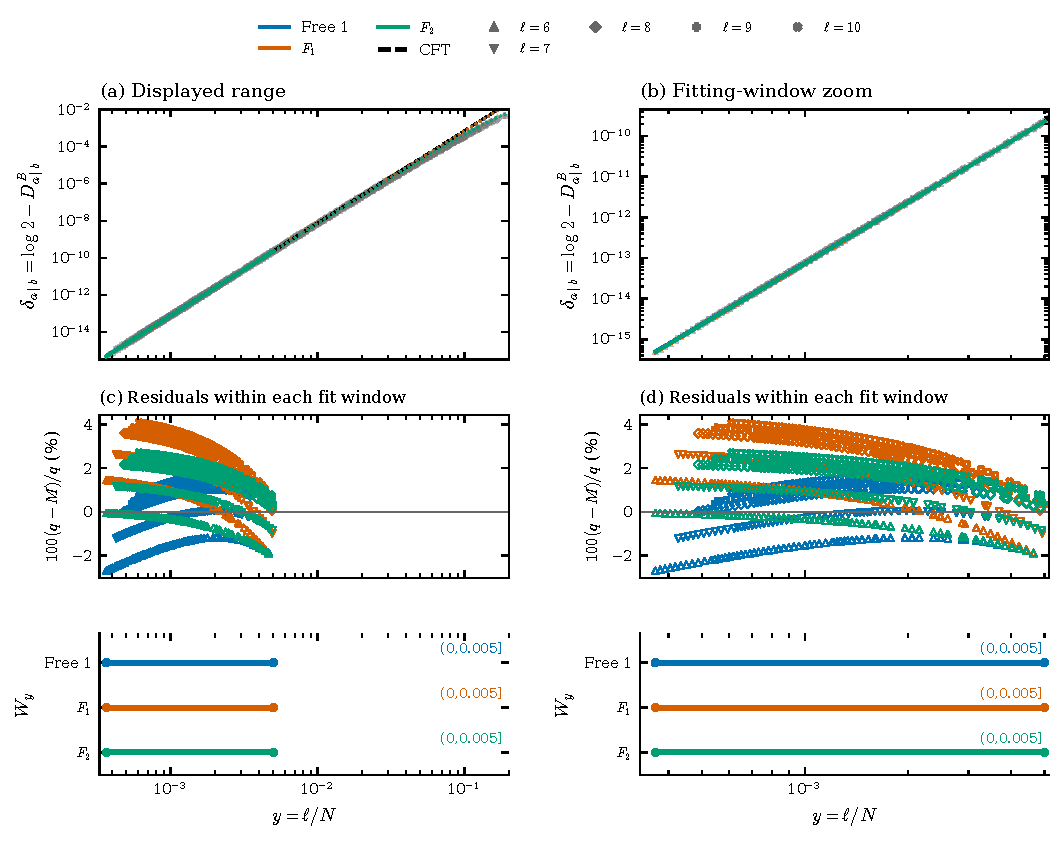
\includegraphics[width=.94\linewidth]{../figs/pair_large_boson_00_3s_s.pdf}\par\smallskip
\begingroup\scriptsize\setlength{\tabcolsep}{4pt}
\begin{tabular}{lllrrrrr}\toprule
Set & Model & $W_z$ & $m$ & $c_0$ & $r^{(0)}$ & $c_1$ & $r^{(1)}$\\\midrule
Both & Free 1 & $(0,0.005]$ & 317 & 66.924 & 4.9836496 & --- & ---\\
Both & $F_1$ & $(0,0.005]$ & 317 & 73.093 & 5 & --- & ---\\
Both & $F_2$ & $(0,0.005]$ & 317 & 74.307 & 5 & -265.58 & 6\\
\midrule
Both & CFT & --- & --- & 75.109 & 5 & --- & ---\\
\bottomrule\end{tabular}
\endgroup
\caption{Compact boson, large intervals, $00\mid 3s,s$, at $p=1/2$, $\ell=6,\ldots,10$, and the complete size grid in Eq.~\eqref{eq:extended-grid}. Here $z=y$ and $q=\delta=\log2-D^B$. Left: all computed data through $z=0.20$; right: a zoom into the common fitting window. Both columns show the same Free 1, $F_1$, and $F_2$ fits. All six directions of this CFT and interval type use the same window. Gray markers denote the data. Colored solid segments lie inside each model\textquotesingle s fitting interval; dotted segments are extrapolations. Black dashed is the analytical CFT leading deficit. The observable axes are logarithmic and span the measured data; nonpositive predictions cannot appear there and out-of-range extrapolations leave the panel. Residual ordinates are linear and show $100(q-M)/q$ only on each model\textquotesingle s fitted observations. Bars give the exact fitting intervals. The parameter block follows Eq.~\eqref{eq:fit}, with $c_0,c_1$ multiplying $z^{r^{(0)}},z^{r^{(1)}}$; all coefficients include powers of $\pi$. A dash means an absent fitted term, or no fitting window for CFT. Values shown are rounded; curves use full precision.}
\label{fig:pair-large_boson-00-3s_s}
\end{figure}
\begin{figure}[!htbp]\centering
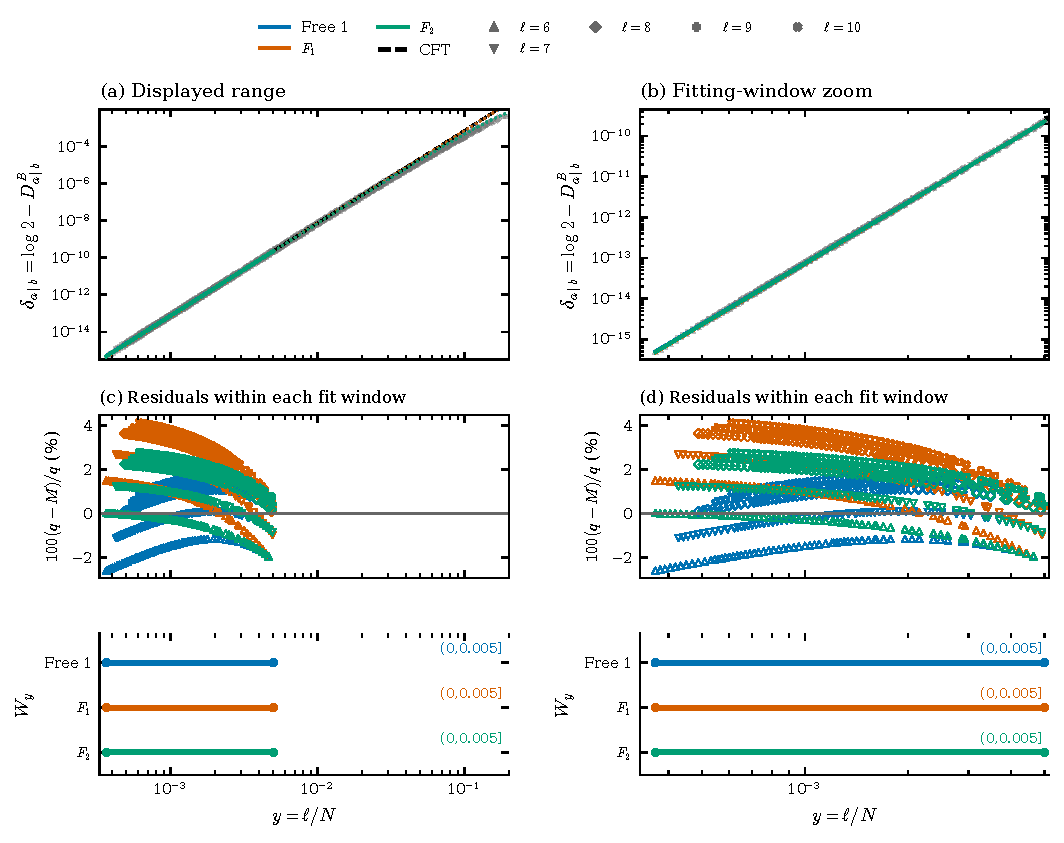
\includegraphics[width=.94\linewidth]{../figs/pair_large_boson_3s_s_00.pdf}\par\smallskip
\begingroup\scriptsize\setlength{\tabcolsep}{4pt}
\begin{tabular}{lllrrrrr}\toprule
Set & Model & $W_z$ & $m$ & $c_0$ & $r^{(0)}$ & $c_1$ & $r^{(1)}$\\\midrule
Both & Free 1 & $(0,0.005]$ & 317 & 66.96 & 4.9838386 & --- & ---\\
Both & $F_1$ & $(0,0.005]$ & 317 & 73.058 & 5 & --- & ---\\
Both & $F_2$ & $(0,0.005]$ & 317 & 74.252 & 5 & -261.18 & 6\\
\midrule
Both & CFT & --- & --- & 75.109 & 5 & --- & ---\\
\bottomrule\end{tabular}
\endgroup
\caption{Compact boson, large intervals, $3s,s\mid 00$, at $p=1/2$, $\ell=6,\ldots,10$, and the complete size grid in Eq.~\eqref{eq:extended-grid}. Here $z=y$ and $q=\delta=\log2-D^B$. Left: all computed data through $z=0.20$; right: a zoom into the common fitting window. Both columns show the same Free 1, $F_1$, and $F_2$ fits. All six directions of this CFT and interval type use the same window. Gray markers denote the data. Colored solid segments lie inside each model\textquotesingle s fitting interval; dotted segments are extrapolations. Black dashed is the analytical CFT leading deficit. The observable axes are logarithmic and span the measured data; nonpositive predictions cannot appear there and out-of-range extrapolations leave the panel. Residual ordinates are linear and show $100(q-M)/q$ only on each model\textquotesingle s fitted observations. Bars give the exact fitting intervals. The parameter block follows Eq.~\eqref{eq:fit}, with $c_0,c_1$ multiplying $z^{r^{(0)}},z^{r^{(1)}}$; all coefficients include powers of $\pi$. A dash means an absent fitted term, or no fitting window for CFT. Values shown are rounded; curves use full precision.}
\label{fig:pair-large_boson-3s_s-00}
\end{figure}
\begin{figure}[!htbp]\centering
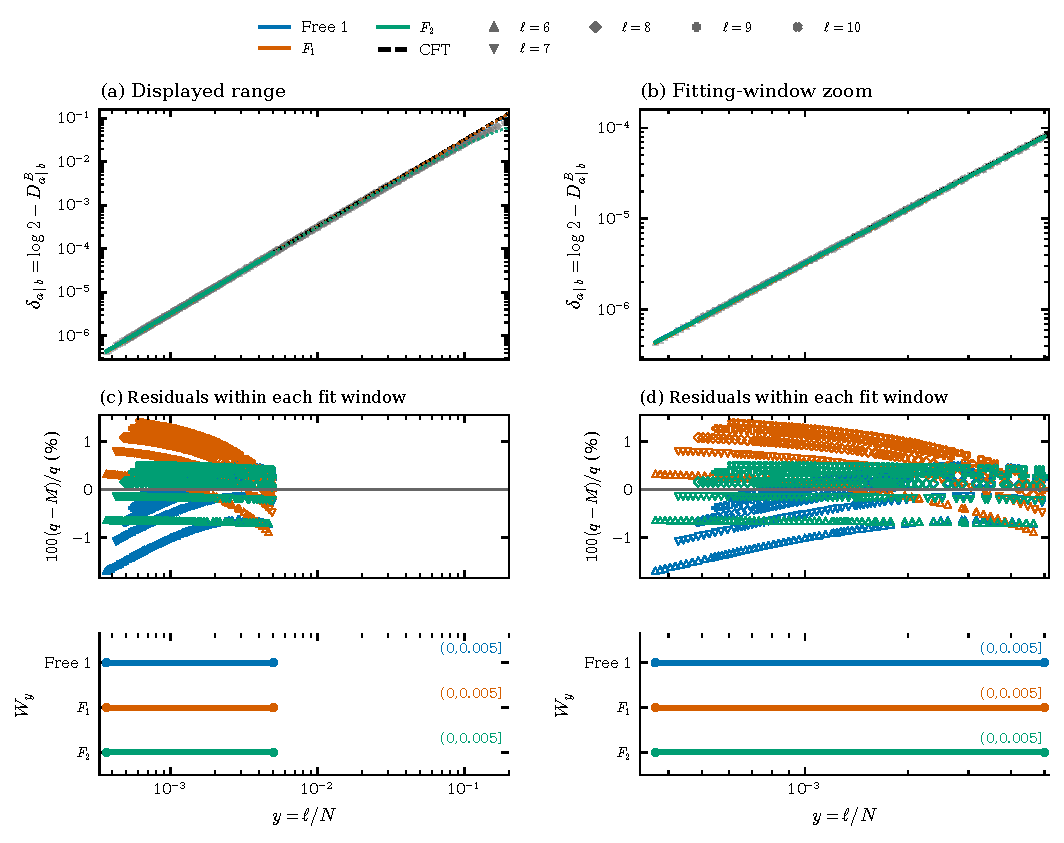
\includegraphics[width=.94\linewidth]{../figs/pair_large_boson_ss_3s_s.pdf}\par\smallskip
\begingroup\scriptsize\setlength{\tabcolsep}{4pt}
\begin{tabular}{lllrrrrr}\toprule
Set & Model & $W_z$ & $m$ & $c_0$ & $r^{(0)}$ & $c_1$ & $r^{(1)}$\\\midrule
Both & Free 1 & $(0,0.005]$ & 317 & 3.069 & 1.9914473 & --- & ---\\
Both & $F_1$ & $(0,0.005]$ & 317 & 3.2185 & 2 & --- & ---\\
Both & $F_2$ & $(0,0.005]$ & 317 & 3.2529 & 2 & -8.6617 & 3\\
\midrule
Both & CFT & --- & --- & 3.2899 & 2 & --- & ---\\
\bottomrule\end{tabular}
\endgroup
\caption{Compact boson, large intervals, $ss\mid 3s,s$, at $p=1/2$, $\ell=6,\ldots,10$, and the complete size grid in Eq.~\eqref{eq:extended-grid}. Here $z=y$ and $q=\delta=\log2-D^B$. Left: all computed data through $z=0.20$; right: a zoom into the common fitting window. Both columns show the same Free 1, $F_1$, and $F_2$ fits. All six directions of this CFT and interval type use the same window. Gray markers denote the data. Colored solid segments lie inside each model\textquotesingle s fitting interval; dotted segments are extrapolations. Black dashed is the analytical CFT leading deficit. The observable axes are logarithmic and span the measured data; nonpositive predictions cannot appear there and out-of-range extrapolations leave the panel. Residual ordinates are linear and show $100(q-M)/q$ only on each model\textquotesingle s fitted observations. Bars give the exact fitting intervals. The parameter block follows Eq.~\eqref{eq:fit}, with $c_0,c_1$ multiplying $z^{r^{(0)}},z^{r^{(1)}}$; all coefficients include powers of $\pi$. A dash means an absent fitted term, or no fitting window for CFT. Values shown are rounded; curves use full precision.}
\label{fig:pair-large_boson-ss-3s_s}
\end{figure}
\begin{figure}[!htbp]\centering
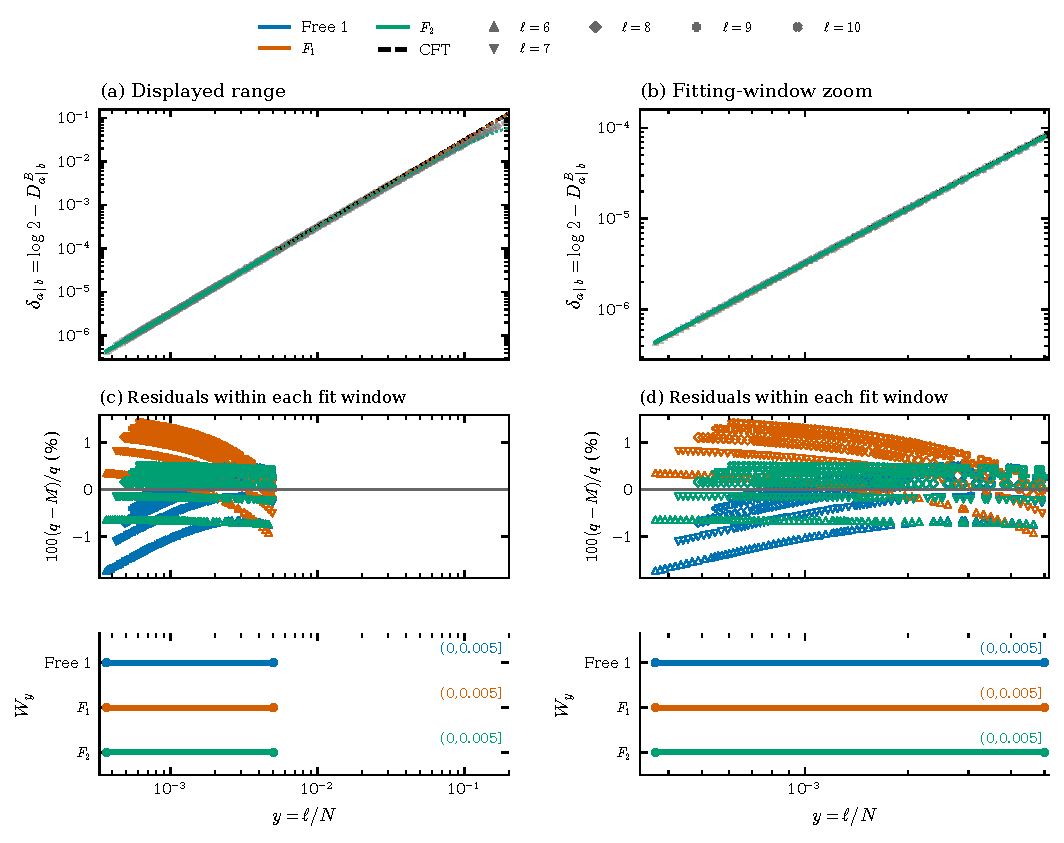
\includegraphics[width=.94\linewidth]{../figs/pair_large_boson_3s_s_ss.pdf}\par\smallskip
\begingroup\scriptsize\setlength{\tabcolsep}{4pt}
\begin{tabular}{lllrrrrr}\toprule
Set & Model & $W_z$ & $m$ & $c_0$ & $r^{(0)}$ & $c_1$ & $r^{(1)}$\\\midrule
Both & Free 1 & $(0,0.005]$ & 317 & 3.0643 & 1.9912306 & --- & ---\\
Both & $F_1$ & $(0,0.005]$ & 317 & 3.2176 & 2 & --- & ---\\
Both & $F_2$ & $(0,0.005]$ & 317 & 3.2528 & 2 & -8.8758 & 3\\
\midrule
Both & CFT & --- & --- & 3.2899 & 2 & --- & ---\\
\bottomrule\end{tabular}
\endgroup
\caption{Compact boson, large intervals, $3s,s\mid ss$, at $p=1/2$, $\ell=6,\ldots,10$, and the complete size grid in Eq.~\eqref{eq:extended-grid}. Here $z=y$ and $q=\delta=\log2-D^B$. Left: all computed data through $z=0.20$; right: a zoom into the common fitting window. Both columns show the same Free 1, $F_1$, and $F_2$ fits. All six directions of this CFT and interval type use the same window. Gray markers denote the data. Colored solid segments lie inside each model\textquotesingle s fitting interval; dotted segments are extrapolations. Black dashed is the analytical CFT leading deficit. The observable axes are logarithmic and span the measured data; nonpositive predictions cannot appear there and out-of-range extrapolations leave the panel. Residual ordinates are linear and show $100(q-M)/q$ only on each model\textquotesingle s fitted observations. Bars give the exact fitting intervals. The parameter block follows Eq.~\eqref{eq:fit}, with $c_0,c_1$ multiplying $z^{r^{(0)}},z^{r^{(1)}}$; all coefficients include powers of $\pi$. A dash means an absent fitted term, or no fitting window for CFT. Values shown are rounded; curves use full precision.}
\label{fig:pair-large_boson-3s_s-ss}
\end{figure}

